% define document type (i.e., template. Here: A4 APA manuscript with 12pt font)
\documentclass[man, 12pt, a4paper, mask]{apa7}

% change margins (e.g., for margin comments):
%\usepackage{geometry}
% \geometry{
% a4paper,
% marginparwidth=30mm,
% right=50mm,
%}

% add packages
\usepackage[american]{babel}
\usepackage[utf8]{inputenc}
\usepackage{csquotes}
\usepackage{hyperref}
\usepackage[style=apa, sortcites=true, sorting=nyt, backend=biber, natbib=true, uniquename=false, uniquelist=false, useprefix=true]{biblatex}
\usepackage{authblk}
\usepackage{graphicx}
\usepackage{setspace,caption}
\usepackage{subcaption}
\usepackage{enumitem}
\usepackage{lipsum}
\usepackage{soul}
\usepackage{xcolor}
\usepackage{fourier}
\usepackage{stackengine}
\usepackage{scalerel}
\usepackage{fontawesome}
\usepackage[normalem]{ulem}
% \usepackage{longtable}
\usepackage{amsmath}
\usepackage{afterpage}
\usepackage{float}
\usepackage{array}
\usepackage{rotating}
\usepackage{censor}

% add definition sections
\newtheorem{definition}{Definition}
\newcommand{\defref}[2][]{\hyperref[#2]{Definition \ref*{#2}#1}}

% Select what to do with to-do notes: 
% \usepackage[disable]{todonotes} % notes not showed
% \usepackage[draft]{todonotes}   % notes showed

% make warning with red triangle
\newcommand\Warning[1][2ex]{%
  \renewcommand\stacktype{L}%
  \scaleto{\stackon[1.3pt]{\color{red}$\triangle$}{\tiny\bfseries !}}{#1}}%

% make question with red triangle
\newcommand\Question[1][2ex]{%
  \renewcommand\stacktype{L}%
  \scaleto{\stackon[1.3pt]{\color{red}$\triangle$}{\tiny\bfseries ?}}{#1}}%

% formatting links in the PDF file
\hypersetup{
pdfpagemode={UseOutlines},
bookmarksopen=true,
bookmarksopenlevel=0,
hypertexnames=false,
colorlinks   = true, %Colours links instead of ugly boxes
urlcolor     = blue, %Colour for external hyperlinks
linkcolor    = cyan, %Colour of internal links
citecolor   = cyan, %Colour of citations
pdfstartview={FitV},
unicode,
breaklinks=true,
}

% ref labels
\newcommand{\fgrref}[2][]{\hyperref[#2]{Figure \ref*{#2}#1}}
\newcommand{\tblref}[2][]{\hyperref[#2]{Table \ref*{#2}#1}}
\newcommand{\appref}[2][]{\hyperref[#2]{Appendix \ref*{#2}#1}}

% custom open science badge height
\newlength{\badgeheight}
\setlength{\badgeheight}{1em}

% language settings
\DeclareLanguageMapping{american}{american-apa}

% add reference library file
\addbibresource{references.bib}

% Title and header
\title{The Migration Experience: A Conceptual Framework and Systematic Scoping Review of Psychological Acculturation}
\shorttitle{Acculturation Experience Framework}

% Authors
\author[*,1,2]{Jannis Kreienkamp}
\author[1,2]{Laura F. Bringmann}
\author[1,2]{Raili F. Engler}
\author[1,2]{Peter de Jonge}
\author[1,2]{Kai Epstude}
\affiliation{\hfill}
\affil[1]{University of Groningen, Department of Psychology}
\affil[2]{Other affiliations still missing.}


\authornote{
   \addORCIDlink{* Jannis Kreienkamp}{0000-0002-1831-5604}\\
   \addORCIDlink{Laura F. Bringmann}{0000-0002-8091-9935}\\
   \addORCIDlink{Raili F. Engler}{0000-0002-4656-3672}\\
   \addORCIDlink{Peter de Jonge}{0000-0002-0866-6929}\\
   \addORCIDlink{Kai Epstude}{0000-0001-9817-3847}

We have no known conflict of interest to declare. The authors received no specific funding for this work. Source data and  software is available at \url{https://github.com/JannisCodes/acculturation-review} \citep{Kreienkamp2021b}. Protocols, materials, analysis data, and code are available at \url{https://doi.org/10.34894/U988DU} \citep{Kreienkamp2021a}. 

Correspondence concerning this article should be addressed to Jannis Kreienkamp, Department of Psychology, University of Groningen, Grote Kruisstraat 2/1, 9712 TS Groningen (The Netherlands).  E-mail: j.kreienkamp@rug.nl}

\leftheader{Kreienkamp}

% Abstract
\abstract{
% 150 word version
\noindent\textbf{Academic Abstract}: One of the key challenges to researching psychological acculturation is an immense heterogeneity in theories and measures. These inconsistencies make it difficult to compare past literature, hinder straightforward measurement selections, and stifle theoretical integration. To structure acculturation, we propose to utilize the four basic aspects of human experiences (wanting, feeling, thinking, and doing) as a conceptual framework. We use this framework to build a theory-driven assessment of past theoretical (final \textit{N} = 92), psychometric (final \textit{N} = 233), and empirical literature (final \textit{N} = 530). We find that the framework allows us to examine and compare past conceptualizations. For example, empirical works have understudied the more internal aspects of acculturation (i.e., motivations and feelings) compared to theoretical works. We, then, discuss the framework's novel insights including its temporal resolution, its comprehensive and cross-cultural structure, and how the framework can aid transparent and functional theories, studies, and interventions going forward.

% 250 word version
%One of the key challenges to researching psychological acculturation is an immense heterogeneity in theories and measures. These inconsistencies make it difficult to compare past literature on acculturation, hinder straight-forward measurement selections, and hamper the development of an overarching framework. To structure our understanding of the migration process, we propose to utilize the four basic aspects of human experiences (wanting, feeling, thinking, and doing) as a conceptual framework. We use this framework to build a theory-driven assessment of past theoretical (final \textit{N} = 92), methodological (final \textit{N} = 233) and empirical literature (final \textit{N} = 530). We find that the framework meaningfully structures past research. We, for example, find core differences between the theoretical and applied literature, where empirical works have understudied the more internal aspects of acculturation (motivations and feelings) and have often fallen short of capturing all four aspects of the migration experience. We also show that some publication fields include on fewer experience aspects and focus on different combinations of factors. We, then, discuss the framework's novel insights including its temporal resolution, its comprehensive and cross-cultural structure and how the framework can aid transparent and functional theories, studies, and interventions going forward.

\noindent\textbf{Public Abstract}: This systematic scoping review indicates that the concept of psychological acculturation can be structured in terms of affect (e.g., feeling at home), behavior (e.g., language use), cognition (e.g., ethnic identification), and desire (e.g., independence wish). We find that the framework is useful in structuring past research and helps with new predictions and interventions. We, for example, find a crucial disconnect between theory and practice, which will need to be resolved in the future.

%\noindent\textbf{Citation Statement}: You will be required to include a brief statement about your set of citations as part of your submission.  This statement should comment on the breadth of the citations that are included in your manuscript, with a specific statement about the diversity (broadly construed) of the authors you have cited.
}

\keywords{Psychological Acculturation, Experience, Framework, Systematic scoping Review\\
    \textit{Open Science Practices:}
    \noindent \href{https://osf.io/n587w/?view_only=0809085870604eda8349baa90b4fd3e5}{
\includegraphics[height=\badgeheight]{assets/open-badges-small/material-color.png}} Open Materials, 
    \href{https://osf.io/n587w/?view_only=0809085870604eda8349baa90b4fd3e5}{
\includegraphics[height=\badgeheight]{assets/open-badges-small/data-color.png}} Open Data,
    \href{https://osf.io/n587w/?view_only=0809085870604eda8349baa90b4fd3e5}{
\includegraphics[height=\badgeheight]{assets/open-badges-small/code-color.png}} Open Code, \break
    \href{https://osf.io/n587w/?view_only=0809085870604eda8349baa90b4fd3e5}{
\includegraphics[height=\badgeheight]{assets/open-badges-small/supplements-color.png}} Open Supplements}


% set indentation size
\setlength\parindent{1.27cm}

% Start of the main document:
\begin{document}

% add title information (incl. title page and abstract)
\maketitle

% **CHEAT SHEET / LEGEND**
%
% Comments:
% '%' starts a comment in LaTeX (not printed)
% '\todo[inline]{} makes orange boxes in PDF
% '\marginpar{}' notes in margins
% '\footnote{}' footnote
% '\Warning' important note indicator in PDF (triangle with exclamation mark)
% '\Question' question note indicator in PDF (triangle with question mark)
%
% Citation (with Natbib citation style):
% '\citep[e.g.][p. 15]{CitationKey}' citation in parentheses "(e.g., Berry, 2003, p. 15)"
% '\citet{CitationKey}' citation in text "Berry (2003)"
% '\citealt' and '\citealp' alternate citation without parentheses
% '\citeauthor' and '\citeyear' only year or author
% 
% Headings:
% '\part{}' and '\chapter{}' only relevant for multi-part or multi-chapter documents
% '\section{}' heading level 1
% '\subsection{}' heading level 2
% '\subsubsection{}' heading level 3
% '\paragraph{}' heading level 4
% '\subparagraph{}' heading level 5
%
% formatting:
% '\textbf{}' text bold font
% '\textit{}' text italic font
% '\underline{}' text underline
% '\sout{}' text strike out
% '\textsc{}' text small caps
% '\vspace{1em}' add vertical space
% '\hspace{1em}' add horizontal space
% '\\' new line (i.e., line break)
% '\pagebreak' start new page (i.e., page break)
% '\noindent' do not indent current line (e.g., current paragraph)
% 'begin{center}...end{center}' center text or object
%
% Math mode:
% '$\alpha = .8$' mathematical equation inline
% '$$\hat{y} = b_0 + b_1x$$' mathematical equation in its own line
% '\begin{equation}...\end{equation}' multi-line equation
% '\approx' approximate symbol
% '\neq' not equal
% '\bar' mean bar over letter
% '\pm' plus minus sign 
% '^{}' superscript
% '_{}' subscript
% '\fraq{numerator}{denominator}' fraction
% '\sqrt[n]{}' square root
% '\sum_{k=1}^n' sum for 1 through n
%
% Insert things from elsewhere:
% '\input{filename}' inputs the raw (tex) file as a command (e.g., tables and R-Markdown imports)
% '\include{filename}' includes section on new page (incl. possible auxiliary info)
% '\includegraphics[settings]{filename}' add a figure or graph
% '\caption{}' adds a caption to a table or figure
% '\label{}' labels sections, tables, figures, etc. so that they can be referred to.
% '\ref{}' refer to a labelled sections, tables, figures, etc.
% '\begin{enumerate}...\end{enumerate}' numbered list
% '\begin{itemize}...\end{itemize}' bullet-ed list
% '\item' item in list section 
%
% Symbols:
% '\&' and sign
% '\%' percent sign
% '\_' three dotes
% '\#' hash symbol
% ------------------------------------------------------------------


% Relevance
% Long discussed and relevant to society
The question of how people change when they get into continuous first-hand contact with other cultures is likely as old as the history of human migration. And thus migration adjustment remains an important issue for many societies around the world. 
Over the past 80 years, researchers of the psychological sciences have proposed hundreds of models and measurements for this phenomenon of "psychological acculturation" \citep[][]{Rudmin2003a}. Yet, despite enormous theoretical and empirical advances, it remains unclear what psychological acculturation exactly entails and a conceptual framework allowing for a synthesis of the past literature on psychological acculturation is still missing \citep{Birman2014c}.

% Problem - Illustration: Past Theory Use
We find an illustration of this challenging heterogeneity in the use of prominent theories of psychological acculturation. One prominent approach has been to conceptualize psychological acculturation as a two-dimensional set of orientations towards the heritage- and the dominant culture --- Berry's (\citeyear{Berry1980, Berry1997b, Berry2005}) now famous `acculturation orientations'. However, over the past 40 years, Berry himself has used a variety of attitudes (i.e., preferences) and behaviors (i.e., actual activities) to describe what these orientations should entail \citep{Berry2005}. And a broader review of the theory found that other researchers had conceptualized and measured `acculturation orientations' with even more diverse aspects. Conceptualizations had, for example, included attitudes, attachments, goals, identifications, or choices and uses of cultural elements \citep[e.g., language, food, or dresses. See,][]{Rudmin2003a}. We see a similar pattern with conceptualizations of psychological acculturation as a `psychological and socio-cultural adaptation' process. Here, cultural adaptation has, for example, included aspects such as life satisfaction and well-being, as well as cultural skills, and work performance \citep{Searle1990, Ward2001, Berry2003}.
Measurements of psychological acculturation are, thus, inconsistent across studies and it remains unclear what aspects the concept exactly entails, and how these aspects are organized.

% Problem - Consequences
% Theory and Application; Past and Future
This heterogeneity of aspects presents fundamental challenges to researchers, practitioners, and policy-makers in the field. Looking back at past theories and measures, different conceptualizations might lead to different results \citep{Snauwaert2003} and the diversities of included or excluded concepts makes it virtually impossible to compare different studies --- which makes it difficult to integrate them quantitatively or qualitatively \citep{Taft1981}.
And looking forward, it remains difficult to select acculturation elements and develop new theories and measurements. A coherent conceptual framework would be necessary to make informed and transparent choices about which aspects are (ir)relevant to a given research question and how they relate to one another.
Given these challenges, some have even suggested that psychological acculturation should not be measured until common terminologies and frameworks are available \citep{Escobar2000}.

% Aim - General
% Therefore we suggest a conceptual framework
We have, thus, developed a descriptive conceptual framework to disentangle, compare, and organize the many conceptual elements found within the literature. In this paper, we describe how this framework was developed based on recent developments within the literature and how the framework gives space to the complexities of psychological acculturation. We then apply the framework in a systematic scoping review of the literature to examine its utility and identify gaps within the literature. The proposed framework, thus, has a different objective than previous efforts which have cataloged literature on acculturation \citep[e.g.,][]{Castels2003}, built multidimensional measures of integration \citep[e.g.,][]{Harder2018}, normative frameworks \citep[e.g.,][]{Ager2008a}, or theories of acculturation \citep[e.g.,][]{Berry2005}. Rather than offering a new measurement, definition, or theory, we aim to build a framework to assess, organize, and compare these conceptual elements. 

% Aim - Specific
% We do this by using ABCD
To build a framework that gives space to the contextual complexity of psychological acculturation while structuring the concept across a wide range of contexts, we propose to utilize the basic aspects of human experiences. Bringing together the rich empirical literature and building on past reviews, we propose that the psychological acculturation experience can be understood in terms of affects, behaviors, cognitions, and desires. Psychological acculturation in this framework might, for example, be understood or measured in terms of behavioral acculturation, such as language use, or voting; cognitive acculturation, such as ethnic identification, or cultural values endorsement; affective acculturation, such as feeling at home, or loneliness; motivational acculturation, such as the satisfaction of competence or independence needs; or as a combination of any or all of these aspects (also see \tblref{tab:AspectExamples} for a range of example concepts). 

Such a framework, thus, explicitly aims to allow researchers and practitioners to review past acculturation literature based on the aspects considered. As a result, researchers can consider broader integration efforts and novel predictions of how acculturation processes develop psychologically. Moreover, the affect, behavior, cognition, desire separation allows researchers to make clearer and more transparent decisions about which aspects of acculturation are relevant to their research question and which aspects they measure. Similarly, practitioners can use the framework to make more informed decisions on which aspects are relevant for policy development and intervention design. 

Importantly, this structural effort seeks to showcase the conceptual complexity and gives space to contextual idiosyncrasies rather than diminishing or reducing migration experiences. We hope to give prominence to the diversity of conceptual aspects that are relevant to the lived realities of migrants and other acculturating individuals. We offer the ABCD framework as a transferable structure to transparently address the similarities and shared mechanisms but also highlight the complexity and diversity of the full migration experience.

% Structure of Paper
In the following sections, we will develop this framework in more detail and will then apply it in a systematic scoping review of the past theoretical, psychometric, and empirical literature on acculturation.

\begin{table}%[hbt]
\caption{Examples of Coding Levels for the Experience Framework of Psychological Acculturation.}
\label{tab:AspectExamples} 
\begin{tabular}{>{\raggedright\arraybackslash}p{0.15\linewidth} 
>{\raggedright\arraybackslash}p{0.20\linewidth} 
>{\raggedright\arraybackslash}p{0.35\linewidth} 
>{\raggedright\arraybackslash}p{0.25\linewidth}}
\hline 
Aspect & Construct & Concept & Operationalization \\ 
\hline \\ [-0.5em]
Affect & 
Moods \linebreak Emotions \linebreak Feelings \linebreak & 
Loneliness \linebreak Feeling at home \linebreak Satisfaction with life \linebreak Pride \linebreak Comfortableness \linebreak Joy \linebreak Ease \linebreak Well-being \linebreak Worry \linebreak Trust \linebreak & 
"I feel ..." \linebreak "My mood ...." \linebreak "I enjoy ..." \linebreak \\

Behavior & 
Activities \linebreak Habits \linebreak Mannerisms \linebreak & 
Language use \linebreak Civic participation (voting, ...) \linebreak Performance (work, ...) \linebreak Media consumption \linebreak Educational achievement \linebreak Peer contacts \linebreak Food consumption \linebreak Cultural habits (holidays, ...) \linebreak Delinquency \linebreak Marriage \linebreak & 
"I do ..." \linebreak "I speak ..." \linebreak "I meet ..." \linebreak \\ 

Cognition & 
Knowledge \linebreak  Memories \linebreak Evaluations \linebreak & 
Ethnic identification \linebreak Cultural values \linebreak Acculturation orientation \linebreak Preferences (food, friends, ...) \linebreak Knowledge \linebreak Importance ratings \linebreak Inner thought language \linebreak Perceived obligations \linebreak Beliefs \linebreak Stereotypes \linebreak & 
"I prefer ..." \linebreak "I think ..." \linebreak "I identify as ..." \linebreak \\ 

Desire & 
Needs \linebreak Goals \linebreak Wants \linebreak & 
Competence \linebreak Independence \linebreak Self-coherence \linebreak Belonging \linebreak Achievement \linebreak Justice \linebreak Growth \linebreak Respect \linebreak Acceptance \linebreak Identity continuity \linebreak & 
"I want ...",\linebreak "I would like to ..." \linebreak "I need ..." \linebreak \\ 

\hline \\ [-0.75em]
\multicolumn{4}{p{\linewidth}}{\footnotesize \textit{Note.} Some of the concepts might include multiple experience aspects depending on the context.}

\end{tabular}
\end{table}


\section{Framework Development} 
This framework explicitly emerged from recent empirical and theoretical developments within the acculturation field in particular as well as the psychological phenomenological literature more broadly. We were able to benefit from a strong theoretical tradition in the field and the broader conceptual framework we propose arguably brings together many of the past advances in capturing psychological acculturation at different levels of conceptualization. To adequately situate the conceptual framework within the past theoretical and empirical efforts, we will first briefly address the notion of using a phenomenological approach for psychological acculturation. We will then introduce each of the experience aspects as they emerge from the literature on psychological acculturation. As a final step of the framework development, we will discuss which functional characteristics the framework highlights and how these functional elements integrate past theoretical advances.

\subsection{A Phenomenological Perspective}
% Experience Structure
There is a converging theoretical consensus that human experiences can fundamentally be understood in terms of wanting, feeling, thinking, and doing \citep[sometimes referred to as the ABCs or ABCDs of psychology: affect, behavior, cognition, desire; e.g.,][]{Cottam2010, Hogg2005, Jhangiani2014}.\footnote{It should also be noted that ABC(D) frameworks have been used effectively to structure theories and models across a wide variety of fields --- including research on attitudes \citep{Breckler1984} and ambivalence \citep{VanHarreveld2015}, the self \citep{Cote2009} and self-regulation \citep{Ben-Eliyahu2015}, the big five personality traits \citep{Wilt2016}, suicidality \citep{Harris2015} and in clinical interventions \citep{Eifert1989}. Interestingly, the affect, behavior, and cognition structure has even found application in the development of human-like machines \citep{Guo2020}.} Following the premise that any human experience can be conceptualized within these four basic aspects, we believe that an ABCD framework of psychological acculturation could offer a comprehensive and theory-driven framework to structure and analyze the many conceptual elements of psychological acculturation. 

However, given the prevalence of ABC(D) structures within the psychological literature in general, it is important to ask how the affect, behavior, cognition, and desire aspects are conceptually relevant to psychological acculturation in particular. To address the conceptual relevance of the four aspects, we look at two common definitions of (psychological) acculturation to identify the conceptual contexts of psychological acculturation. Firstly, the Social Science Research Council originally defined the broader concept of \textit{acculturation} as:
\begin{definition}[Acculturation]\label{def:acculturation}
Acculturation comprehends those phenomena which result when groups of individuals having different cultures come into continuous first-hand contact, with subsequent changes in the original culture patterns of either or both groups.

\hfill--- \citealp[][]{Redfield1936}; p. 149
\end{definition}
From the broader concept, the individual level experience of \textit{psychological adaptation} --- which is the focus of the present framework --- has commonly been further specified as:
\begin{definition}[Psychological Acculturation]\label{def:psychAcculturation}
Psychological acculturation refers to the changes an individual experiences as a result of being in contact with other cultures, or participating in the acculturation that one’s cultural or ethnic group is undergoing \citep[][]{Graves1967}. 
    
\hfill--- as cited in \citealp[][]{Sam2006}; p. 14
\end{definition}

Within both of these definitions, psychological acculturation, thus, fundamentally comprehends any individual changes as the result of cultures and contacts. The different types of individual-level \textit{phenomena} and \textit{changes} are the topic of this framework but the prerequisites of \textit{culture} and \textit{contact} are central to understanding how the psychological experience emerges. We will, thus, briefly discuss how we conceptualize cultures and contact within the framework and how that aligns with the ABCD structure of the individual experience.
    
\subsubsection{Culture}
% Culture
To discuss the role of cultures, we will look at one last definition. In this framework, we follow the approach refined by \citet[][]{adams2004}, which defines cultures as cultural patterns:
\begin{definition}[Culture]\label{def:culture}
Culture consists of explicit and implicit patterns of historically derived and selected ideas and their embodiment in institutions, practices, and artifacts; cultural patterns may, on one hand, be considered as products of action, and on the other as conditioning elements of further action. \citep[based on][p. 181]{kroeber1952}. 

\hfill--- as cited in \citealp[][]{adams2004}; p. 341
\end{definition}

This definition highlights a number of features that are central to our efforts of conceptualizing psychological acculturation. In particular, the definition emphasizes that cultural patterns (1) are dynamically changing over time (i.e., are historically derived), (2) are agentically re-produced (i.e., selected ideas), and (3) dualistically reside both in the individual (i.e., who produces the patterns) as well as the physical and social context \citep[i.e., which embodies and conditions;][]{adams2004}. As such, the definition follows the general tenets that are shared by many theoreticians within the acculturation field \citep[e.g., see][]{Berry2009, Ward2016}. At the same time, however, in empirical practice models of acculturation have often focused on cultures as static, externalized influences \citep[e.g., see the commonly (mis-)used models of][]{Berry1997b, Berry2006a}. We argue that affects, behaviors, cognitions, and desires connect the external embodiments and conditionings of cultural patterns with the individual choice of which cultural patterns will be reproduced. 
    
Within the sociological literature, the external social influences of cultures can be divided into formal social facts (e.g., laws, regulations, policies, history, language), informal social facts \citep[e.g., norms, values, beliefs, rituals, customs; also see][]{Herzog2018}, as well as more material cultural products or artifacts \citep[e.g., food, fashion, architecture, or arts, such as film, music, literature, and fine arts; e.g., see][]{Alexander2001}. The content of these external influences often formally or informally embodies expected patterns of behavior (e.g., dress or communication styles), cognition (e.g., sense of race-, class-, gender-, and sexual identities), emotions (e.g., expressions of emotions), and motivations (e.g., virtues and duties).

At the same time, however, affect, behaviors, cognitions, and desires also drive what we consider `cultures' to be \citep[e.g.,][]{Varnum2017}. For example, cultural knowledge, values, identities, beliefs, and attitudes are likely the most widely discussed aspects of non-material cultural patterns \citep[i.e., cognitions; e.g.,][]{DiMaggio1997}, several indigenous cultural practices are legally protected as manifestations of culture \citep[i.e., behaviors; e.g., Art. 11][]{UnitedNations2007}, shared emotions are an integral part of culture creation in narratives \citep[i.e., affects; e.g.,][]{Ahmed2014, Kitayama1994, Smith2016c, Sundararajan2015}, and motivational ideals or oughts form the basis of many cultural discussions \citep[i.e., desires; e.g., see][]{Markus1991}.

In the case of psychological acculturation, a migrating individual needs to deal with (at least) two sets of cultural patterns --- the heritage cultural patterns and any local cultural patterns \citep[e.g., see][]{Ferguson2015}. The individual will, thus, have to negotiate their individual response to the cultural expectations of the cultural patterns of their new context and their own held cultural patterns. These individual responses in affects, behaviors, cognitions, and desires thus impeccably connect internal and external cultural patterns as they actively evolve over time \citep[also see the psychological foundations of culture, in][]{adams2004}. In other words, the psychological acculturation experience (i.e., the individual experience of ABCD) captures the adjustment to tension as a result of different patterns of internal, shared, and embodied affects, behaviors, cognitions, and desires. Moreover, studying psychological acculturation in the experience framework then also allows us to reflect on which cultural patterns are in positions of power \citep{Bhatia2001}.

% Adaptation
Additionally, affect, behavior, cognition, and desire have all been highlighted in the conceptualization of human functioning and adaptation to conflicting cultural patterns --- a core outcome for many acculturation researchers \citep[e.g., see][]{Berry2006a, Searle1990, Ward2001, Maertz2016}. Adaptation in such an understanding can include, behavioral adaptions, such as building skills and competencies \citep[e.g.,][]{Bevan1965}, cognitive adaptation, including self-image restorations and dissonance reductions \citep[e.g.,][]{Czajkowska2017}, affective adaptions, such as dealing with feelings of culture shock and homesickness \citep[e.g.,][]{Smith1990, VanTilburg1996}, as well as desire adaptations, such as regulations of status and affection needs \citep[e.g.,][]{Steverink2006}. In short, affects, behaviors, cognitions, and desires not only form the fundamental aspects of human experiences but also connect the external and internal cultural patterns in such a way that they showcase the nuances of dynamic, agentic, and adaptive (re-)productions of the cultural patterns that underlie acculturation.

\subsubsection{Contact}
Beyond the cultural contextualization, it is also important to consider the contacts that drive cultural adaptation. One way of structuring the situational contact contexts is what we will here refer to as the \textit{domains of psycho-social functioning} --- the idea that the social experience will take place within different domains in life. There are many social-scientific theories that have discussed these spheres of life. One famous example is Bronfenbrenner's Ecological systems theory \citep{Bronfenbrenner1992}, according to which humans get into contact with others, and society at large, through a number of environmental systems that range from the closest relations (e.g., family or colleagues) to the more remote relationships (e.g., mass media or societal services). A similar framework was suggested by prominent theorists of the (structural) functionalist traditions with the concept of social institutions \citep[e.g.,][]{Turner1997}. According to these sociological theorists, it is through societal institutions (commonly: family, government, economy, media, education, healthcare, and religion) that cultural patterns are transmitted and maintained \citep[e.g.,][]{Durkheim1982}. Similar ideas for domains of interaction with society and culture have also been proposed within the acculturation literature. \citet{Arends-Toth2006, Arends-Toth2007} have, for example, suggested 15 public and private life domains (e.g., education [public], child-rearing [private]) in which cultural contact takes place. Empirical research in the individual acculturation field has also provided evidence that acculturation processes can develop separately and differently within these contact domains \citep[e.g.,][]{Arends-Toth2003a}. 

% Interaction
Importantly for our framework, these situational domains afford different affects, behaviors, cognitions, and desires. The contact domain and situation structure which experiences are appropriate or even possible \citep[e.g.,][]{cantor1994}. These situational affordances can be physical, where certain cultural patterns are not possible \citep[e.g., localized ancestral worship][]{kawano2005}; formal, where certain cultural patterns are not allowed \citep[e.g., indigenous hunting practices][]{blaser2009}; or informal where certain cultural patterns are not wanted \citep[e.g., discrimination of black hair][]{robinson2011}. Also more implicitly, empirical studies have, for example, found that cultural contexts differ in the frequency and variety of situations that afford different types of negative social emotions \citep[][]{boiger2013}. Situational affordances, thus, particularly interact with cultural norms and patterns to allow for specific acculturation experiences. These situational affordances in a cultural space then also highlight how power over the situation translates into power over the experiences of acculturating individuals \citep[e.g.,][]{guinote2008}. And more broadly, the individual experience affect, behavior, cognition, and desire as psychological acculturation is embedded within contact structures and captures the situational affordances.

Affect, behavior, cognition, and desire are also embedded within the literature on inter-group and inter-cultural contact in general. How and why people get into behavioral contact with people from other backgrounds has, for example, been linked to group-specific needs, and desires, such as power and acceptance \citep[e.g.,][]{Hassler2021, Shnabel2008a}. Similarly, outcomes of these interactions are often governed by inter-group cognitions, such as perceptions of threat or shared identities \citep[e.g.,][]{Dovidio2017, Stephan2000a} and inter-group emotions, including pride, or anxiety \citep[e.g.,][]{Iyer2008, Stephan1992}. Affect, behavior, cognition, and desire are, thus, also at the very heart of contact with different cultural contexts.

In short, the individual affect, behavior, cognition, and desire aspects are generally well-equipped to address the prerequisite contextual elements of acculturation. In the next sections, we will focus in on the individual psychological acculturation experience and discuss how each of the psychological aspects emerged out of the empirical and theoretical developments within the field. 

\subsection{Affect, Behavior, Cognition, and Desire within the Acculturation Literature}
% ABC in Theoretical Traditions
Interestingly, the ABC structure is not entirely foreign to the field of acculturation. Ward and colleagues \citep{Ward2001, Masgoret2006, Ward2019} have previously pointed out that theoretical perspectives on acculturation tend to focus on affect, behavior, or cognition. Within the affective tradition, Ward situates the stress and coping literature, behavioral traditions are the cultural learning theories, and social identification theories form the cognitive theories. \citet{Sam2006b} has even noted that such a perspective might be useful in structuring the core components of psychological acculturation more broadly. 
Following Sam's (\citeyear{Sam2006b}) suggestion, we propose that, once we include desires (i.e., motivational literature), we can build a generalized conceptual framework. That is to say, the full ABCD structure would not only summarize theoretical traditions but would offer a theory-based framework for the conceptual elements because it comprehensively structures the concept based on the fundamental aspects of a culturally-embedded contact experience. Such a framework should structure psychological acculturation at any level of abstraction --- from the most abstract theory level to the most applied operationalization level. 

Given the centrality of the four aspects to the framework, we will briefly discuss how each of the four aspects are reflected in recent debates within the literature on psychological acculturation. To illustrate how the conceptual ideas are embodied in lived realities, we will additionally provide emblematic quotes from a focus group we conducted as part of the broader project. The focus group discussion is not an empirical part of the framework but rather offers an illustration of the real-world relevance of the individual aspects \citep[the full account of the focus group discussion is available as a separate publication by ][]{kreienkamp2023Blinded}.

\subsubsection{Behavior}
% Behavior and cultural contact
Behaviors --- that is actions and mannerisms --- are often the most overtly and externally visible aspect of the human experience. As such, especially social behaviors (e.g., language learning and contacts outside the home) are visible and reciprocal elements that are deeply connected to cultural contacts \citep[e.g.,][]{Legare2019, Whiting1980, imai2016}.

\begin{displayquote}
    Maria:\\
    {[...]} \textit{while, of course, you integrate best when you go to work.}
    
    Moderator:\\
    \textit{Why is that exactly?}
    
    Maria:\\
    {[...]} \textit{Because there you have daily contacts with locals.}
\end{displayquote}

% Past literature
Given the overt nature of behaviors and their interconnectedness with culture, behaviors have also been a prominent aspect in the acculturation literature. Ward and colleagues (\citeyear{Ward2019}) in their review have identified cultural learning theories as one key literature tradition that has focused on behavioral aspects of acculturation. They relate these learning theories to the acquisition of effective skills and competences as the behavioral operationalizations \citep[including, verbal and non-verbal communication skills][]{Ward2001}. Other examples of behavioral conceptualizations of acculturation (beyond Ward's focus), include civic participation \citep[e.g., voting;][]{Lessard-Phillips2020}, inter-ethnic marriage \citep[e.g.,][]{Song2009}, and media consumption \citep[e.g.,][]{Shoemaker1985}. 

\subsubsection{Cognition}
\begin{displayquote}
    Yahya:\\
    {[...]} \textit{Once I started my education, I felt part of society.} {[...]} \textit{That was not the case when I was learning Dutch at the university, at the language school, or at other places before. Only later when I was at school, ... I feel: Okay, now I feel I am really in the Netherlands.}
    
    Joop:\\
    \textit{Why did you not have that at the language school?}
    
    Yahya:\\
    \textit{Because I was only a refugee.}
\end{displayquote}

% Applied Cognitions
Cognitive aspects, which commonly entail the thinking processes of the human experience, often underlie navigational cultural competencies and social identities in dealing with conflicting cultural patterns \citep[][]{Padilla2003}. Language-, social- and communication norms as well as learning about more formal social systems, values, and social rules are examples of how cognitive changes related to bridging social gaps \citep[e.g.,][]{Gelfand2011, Nisbett2002}. Similarly, both a break in identity (the struggle of defining oneself in the new environment) as well as the struggle of dealing with a singular (migrant or refugee) identity label and the process of developing a more complex identity narrative towards others are applied examples of how cognitions sit at the forefront of adapting to conflicting cultural patterns \citep[e.g.,][]{Verkuyten2012}.

% Past literature
Given the pertinent connection between cultures and cognitive processes, cognitions have also played a major role in the theoretical acculturation literature. Within the cognitive tradition, Ward and colleagues (\citeyear{Ward2001, Ward2019}) have identified ethnic identity and group perception theories, with a particular focus on Berry's (\citeyear{Berry1997b}) acculturation attitudes. Beyond the theories identified by Ward, the acculturation literature has recently also focused on several other cognitive conceptualizations of psychological acculturation, including cultural values \citep[e.g.,][]{Marin2003} and stereotypes \citep[e.g.,][]{Stanciu2018}. 

\subsubsection{Affect}
\begin{displayquote}
    Fariq:\\
    {[...]} \textit{But for me the language is very very difficult. And then you think people are not open. And you don't understand because your language isn't that good. And then I maybe don't feel welcomed when I have questions or want to approach them.}
\end{displayquote}

% Affect highlights individuals
Affect --- the human capacity to feel \citep[including emotions and moods;][]{FeldmanBarrett2007} --- foreground the importance of the subjective experience as acculturation \citep[][]{Holodynski2012}. Instead of focusing on purely behavioral outcome conceptualizations (e.g., housing, job, education), affective acculturation experiences (e.g., feeling at home, feeling accepted) highlight the individual embeddedness components of healthily adapting in a new social environment \citep[][]{mesquita2016}. 

% Past literature
But affect and emotion have also been discussed within the psychological acculturation literature. \citet{Ward2001} in her review of the acculturation traditions, describes the stress and coping literature --- especially Berry's concept of acculturation stress \citep{Berry1997b} --- as the affect component of acculturation. In this tradition, the main constructs that constitute the affective dimension are the psychological and emotional well-being as part of the psychological adaptation process \citep[including, for example, life satisfaction and depression;][]{Ward2019}. However, beyond the theoretical stress literature tradition, there are also more immediate models and measurements of emotional acculturation. There is, for example, a relatively young tradition of 'emotional acculturation' as a distinct concept in which acculturation is understood as the similarity in emotional patterns \citep[see][for a review]{DeLeersnyder2017}. But also individual emotions, such as 'feeling accepted' \citep{Jasini2018}, or 'pride' \citep{Suinn1995} have received attention as discrete conceptualizations of acculturation. 

\subsubsection{Desire}
\begin{displayquote}
    Yahya:\\
    {[...]} \textit{Yes, they [parents] have control like a boss or a god. And I still had that in Syria but it kind of stopped, ... because I am not gonna be a kind of a slave to my family, ... because I want freedom for myself.}
\end{displayquote}

% Focus group discussion
Desires --- the motivational forces of the human experience --- often highlight the individual agency and the deeply functional essence of the acculturation processes \citep[][]{gezentsvey2008}. The needs for interactions, to be understood, for purpose, and for identity continuity are not necessarily expected by the dominant group but are intrinsic and fundamental to the health and functioning of the newcomers during the acculturation process \citep[e.g.,][]{Anzaldua1987}. As deeply internal aspects of the human experience, motivations often also have the potential of fundamentally organizing the manner in which a migrant approaches a new cultural context \citep[][]{vishkin2021, kashima2014}. 

% Past literature
Yet, despite these functional and interconnected properties, few of the past reviews have examined motivation as a distinct aspect of psychological acculturation within the literature or the concept. However, outside of reviews, needs and wants have been discussed more frequently as a conceptual aspect of psychological acculturation. For example, more and more researchers are looking at the motivations for migration in understanding acculturation \citep{Sandu2018, Echterhoff2020}. Additionally, motivations are more frequently considered as underlying  acculturation orientations \citep{Recker2017a}, acculturation behavior \citep{Reece2000}, and psychological adaptation \citep{Safdar2003}. 

\subsection{Functional Embeddedness}
Before we move to the application of the framework in the systematic scoping review, we will discuss a number of functional characteristics that allow the framework to be embedded within real-life experiences and assist in building a deeper theoretical understanding of psychological acculturation.

\subsubsection{Aspect Distinctiveness}
% Experience aspects and lived experience
Firstly, while we have introduced the four experience aspects as distinct elements, it is important to note that both in theory and in practice affect, behavior, cognition, and desire are not experienced as distinct entities. This aspect-interconnectedness is also reflected in theories on the aspects. As an example, most affects have a cognitive component just as most cognitions have an affective value. Similarly, motivation is commonly conceived as having both emotional (e.g., desire) and cognitive (e.g., goals) aspects, both of which are often directed towards behaviors (i.e., conation). Muddying the waters further is the difficulty that many operationalizations (and empirical measures) of psychological acculturation also include multiple aspects. Concepts such as satisfaction or distress, which are common measures of acculturation, famously include affective and cognitive components. Yet, despite the interdependence of aspects in theories and lived experience, the four aspects can consistently be identified within experiences and concepts --- they remain qualitatively different aspects of the experience. And as such, they offer a pragmatic lens to structure the psychological acculturation concept \citep{Kuhn1962}. Differentiating the four (needing, feeling, thinking, and doing) qualities of an experience in what we consider psychological acculturation to be, allows us to structure our discussions of past, current, and future theories and measures of psychological acculturation.

\subsubsection{Experience Content}
Secondly, it is also important to note here that while anyone will have motives, emotions, thoughts, and behaviors, what one needs (e.g., belongingness or independence), feels (e.g., sadness or happiness), thinks (e.g., identification or disinterest), or does (e.g., studying or working) is highly ideographic. It is this ideographic content that makes the framework relevant to such a broad range of migration contexts. Yet, it is the content-free structure --- the presence or absence of the basic aspects in conceptualizations of acculturation --- that is transferable across contexts and studies, enabling comparisons and broader conceptual discussion. It should also be noted that in our view such a framework does not stand in conflict with cultural or indigenous psychological concerns of an absolutist, or deterministic psychology \citep[e.g.,][]{Kim2006a}. In fact, cultural psychologists, together with many decolonial researchers, have long argued that the individual embedded and lived experience should gain a more central role in our theoretical developments \citep[e.g., ontological turn;][]{Pedersen2020}.

\subsubsection{Process}
% Past literature
%% Dynamic process rather than static end-product: 
% Experience can answer this call because it can only be understood based on past experiences
A final, fundamental property we would like to address in the experience framework is the understanding of psychological acculturation as a dynamic process rather than a static end-product. That psychological acculturation is a process, and that ``acculturation occurs when two independent cultural groups come into \textit{continuous first-hand contact over an extended period of time}'' \citep[][186]{Berry1989} seem to be a generally accepted assumption within the field \citep[e.g.,][]{Ward2016}. Yet, some reviews have pointed out that few empirical studies have actually considered the theoretical implications of migration as a process and even fewer have methodologically followed the trajectories of migrants over time \citep[][]{Brown2011, Ward2019}. We believe that the experience framework of psychological acculturation, as it is presented here, is ideally suited to deal with this conceptualization as a process. Philosophers of the phenomenological tradition have long highlighted that a subjective experience can only be understood within the history of past experiences \citep[e.g.,][]{Heidegger1978}. The human experiences are thus scalable and can capture processes of seconds or years and might even relate to generational or future conceptualizations.

As such, the experience structure allows us to integrate, expand, and systematize previous process conceptualizations of psychological acculturation. Working through the many theoretical works within the acculturation literature, we realized that theories focus on one or multiple stages of intercultural contact episodes. This allowed us to integrate theoretical traditions that distinguish between acculturation orientations and later acculturation outcomes \citep[e.g.,][]{TeLindert2008a} and associated methodological efforts that organize different assessments around this division \citep[notably][]{Arends-Toth2006a} with an emerging view that acculturation develops as a series of contact episodes \citep[][]{Maertz2016}. Bringing together several of the terms and approaches used within the literature, we propose to distinguish between (1) acculturation conditions [\textit{ABCDs prior to contact}], (2) acculturation response [\textit{ABCDs during contact}], and (3) acculturation outcome [\textit{ABCDs following the contact}]\footnote{It should again be noted that intercultural contact can either be direct in-person contact or indirect contact through media, institutions, or cultural products.}. 

Importantly, for all three of these steps, different ABCDs can emerge and due to the temporality of these phases, the ABCDs experienced during these three steps are often qualitatively different. As an example, whereas acculturation conditions often focus more on socio-structural and personal expectations, immediate acculturation responses often have a reactive or oppositional character, and acculturation outcomes tend to focus on habitual, reflective, and evaluative experiences in the literature. We discuss these qualitative differences as they are represented in the theoretical literature in more detail during the scoping review below (also see \fgrref{fig:ModelContext} for several example features).

Additionally, by considering the three-stepped process we can also integrate what we call the `conditions of change' and the `conditions of stress' that sit between the three steps. Looking at cultural conflict models \citep[e.g.,][]{Robinson2019}, we can extract a number of conditions based on the presence of differences, evaluations of differences, and external affordances, which determine whether the migrant seeks to change the ABCDs anticipated prior to the contact when they enter the contact \citep[also see][]{Masgoret2006, Alitolppa-Niitamo2004, Grove1985, Wood2014}. Similarly, using stress-adaptation models \citep[e.g.,][]{Kim1988, Hajro2019, Sam2006b}, we are able to discern a number of conditions that address when ABCD changes following the contact lead to stress or adaptation outcomes \citep[also see][]{Ryan2008, Berry1992, Benet-Martinez2005, Salo2015, Wood2014, Hajro2019}. Together, the episodic ABCD approach and the intermittent conditions also highlighted the dynamic, embedded, and circular nature of the cross-cultural contacts at the heart of psychological acculturation (also see \fgrref{fig:ModelContext}).

In sum, the conceptual framework we propose suggests that the concept of psychological acculturation is psychologically fundamentally structured into affect, behavior, cognition, and desire aspects. And while each experiential aspect captured part of the concept, only jointly will they comprehensively capture the full psychological acculturation concept. We have also shown that the four experience aspects are all highly relevant to the concept as they capture the dynamic, adaptive, and interactive functioning of contacts with new cultural patterns. We have further emphasized that the experience framework highlights the embedded complexities of real-world migration experiences and that the distinction of the ABCD structure along the dynamics of cultural contacts brings together several theoretical perspectives of the psychological acculturation literature. 

In practice, the framework can thus find utility in comparing past literature and interventions (e.g., which conceptual aspects were considered for particularly important findings), can structure future study and intervention designs (e.g., which aspects are relevant to health behaviors), and can advance future theoretical developments (e.g., which experiential aspect organizes the other acculturation aspects for specific outcomes). In the following, we will take first steps at exploring the applied utility of the framework, for organizing the past literature on psychological acculturation. 

\begin{sidewaysfigure}
    \centering
    \caption{Conceptual framework of psychological acculturation with context and experience process. The process diagram shows the main elements with examples for each conceptual building block. Note: ABCD = affect, behavior, cognition, desire aspects of psychological acculturation.}
    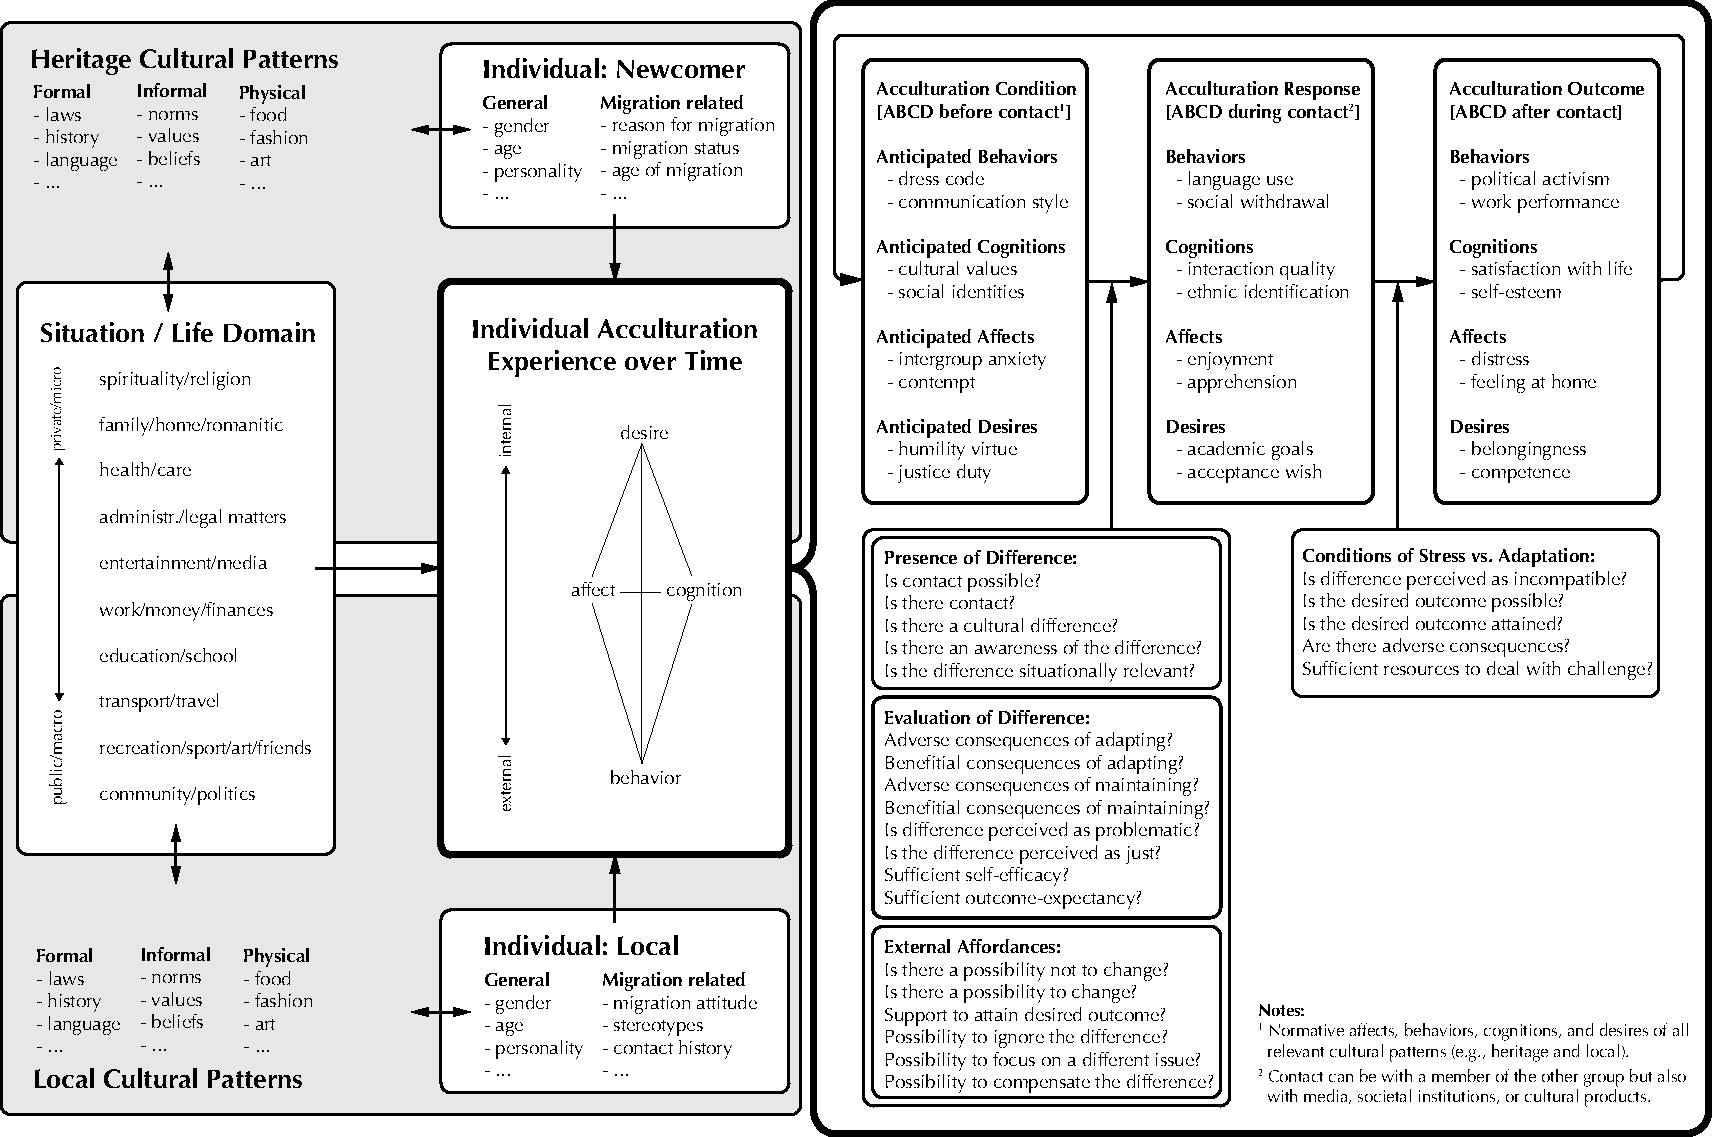
\includegraphics[width=\textwidth]{Figures/ConceptualFrameworkRevision.pdf}
    \label{fig:ModelContext}
\end{sidewaysfigure}

\section{The Present Study}

%\begin{center}
%    \Warning\ \textsc{next sections not re-worked yet} \Warning
%\end{center}

The aim of our empirical efforts presented here is to put our proposed framework to the test. We have lamented that one of the challenges of a heterogeneous field is that it is difficult to assess and compare past literature. As a framework, we have suggested that the psychological aspects of experiences could comprehensively structure our assessment of the literature. We will thus systematically retrieve the past literature on psychological acculturation of first-generation migrants. We chose first-generation migrants specifically to allow for a focused systematic literature search while still maintaining the broad heterogeneity of acculturation experiences. For all relevant works, we will extract which experiential aspects were considered in the research. We expect that these efforts will provide insights into the perceived importance of desires, affects, cognitions, and behaviors for psychological acculturation. We also expect that this allows us to assess how many experience aspects are usually considered and which aspects are considered jointly. And finally, we aim to compare the understanding of psychological acculturation across different fields to assess the comparative utility. 

To apply the framework, we specifically target three bodies of literature that capture the concept of psychological acculturation. Firstly, we will assess the theoretical literature on psychological acculturation. The theoretical literature should offer the broadest, most abstract, and most comprehensive works on psychological acculturation. Coding the aspects considered in these theories should, thus, offer insights into the assumptions on which researchers build their empirical work.
Secondly, we will assess psychometric literature developing acculturation measures. As operationalizations of the construct within the empirical literature, validated scales usually focus on a concept in a generalized manner, rather than focusing on aspects only relevant to a specific `applied' investigation. Coding psychological acculturation measures separately might also aid future considerations of measure selection because we effectively build a database of scales that can be filtered by whether the scale includes measurements of affects, behaviors, cognitions, and desires (see Supplemental Material D). 
Thirdly and finally, once we have considered the validated scales in particular, we will more generally assess the empirical literature that used measures of psychological acculturation. Capturing operationalizations within empirical studies, allows us to investigate the focus within the empirical literature more broadly and allows us to compare differences between fields and research subjects.

In short, the main aims of our empirical efforts can be summarized in four main research questions.
\begin{enumerate}[noitemsep,topsep=0pt,label=RQ \arabic*:,leftmargin=1.8cm]
    \item How have psychological acculturation experiences been conceptualized within the past literature?
    \begin{enumerate}[noitemsep,topsep=0pt,label=(RQ 1\alph*):,leftmargin=1.64cm]
        \item What is the relative importance of each of the affect, behavior, cognition, desire aspects within past conceptualizations?
        \item Which experience aspects are considered jointly in the conceptualization of psychological acculturation?
        \item Which conceptualizations of psychological acculturation cannot be captured with the ABCD framework?
    \end{enumerate}
    \item What are the main differences in the conceptualizations of psychological acculturation experiences across the past theoretical, psychometric, and empirical literature?
    \item How do conceptualizations of psychological acculturation differ in terms of affect, behavior, cognition, and desire aspects across different publication fields?
    \item How is the cultural, individual, and situation context of psychological acculturation conceptualized and addressed in the past literature? [see Supplemental Information E]
\end{enumerate}

To address these research questions we, specifically chose a \textit{systematic scoping review}. Such a review is \textit{systematic} because it uses ``systematic and explicit methods to identify, select, and critically appraise relevant research, and to collect and analyze data from the studies" \citep[PRISMA guidelines; ][p. 1]{Moher2009}. In practice, this meant that we developed systematic a literature search and data extraction protocols for a structured, transparent, and reproducible review (for the systematic search protocol see \appref{app:AppendixSearchStrategy} and for our coding manual see Supplemental Material B; also see \citealp{Peters2015}). To analyze and summarize the data we then perform a \textit{scoping analysis} to ``map the key concepts underpinning a research area and the main sources and types of evidence available" \citep[][p.21]{Arksey2005}. In our case, this meant that we were able to address our broader research questions of how psychological acculturation has been conceptualized within different bodies of past literature and how useful the ABCD separation was in assessing and comparing conceptualizations.

It should also be noted that we consciously chose not to conduct a meta-analysis. We conduct this review exactly because we are worried about comparability across studies, a key requirement of meta-analyses \citep{Pogue1998}. In our case, we, arguably, do not have a clearly defined concept and exclusions to ensure a cohesive data set would be counterproductive to our efforts. Moreover, a meta-analysis is commonly understood as an analysis of analyses \citep{Glass1976}. However, since we are interested in a conceptualization (rather than a relationship, a scale metric, or population parameter) a quantitative summary in form of a meta-analysis is not well-suited to answer our research question. Also a meta-analysis of our own extracted data seems profitless because it would likely mirror a sample size weighted average.

In the following section, we will briefly discuss how we conducted the systematic scoping review and will sequentially analyze the role of experience aspects in the theoretical, psychometric, and empirical literature of psychological psychological acculturation. Please note that all protocols, materials, data, and software code is openly accessible as part of our OSF repository \citep[][]{Kreienkamp2021e}.


\section{Systematic scoping Review}
% import methods and results from R Markdown (in file: "Methods-and-Results.tex")
\newcommand{\nTheo}{92}
\newcommand{\nMeth}{233}
\newcommand{\nEmp}{526}

To assess the past empirical and theoretical literature on psychological
acculturation, we performed a systematic scoping review. We first read
seminal and review works within the field
\citep[including,][]{Ward2019, Berry1997b, Berry2003, Szapocznik1978, Sam2006a, Rudmin2003a}.
Based on our reading of the literature, we designed a comprehensive
literature search strategy in an iterative fashion. For the empirical
work on acculturation we performed a literature search on March
4\textsuperscript{th}, 2020 and February 14\textsuperscript{th}, 2021,
within the ``APA PsycINFO'' bibliographic databases using the
EBSCO\textit{host} provider. The databases also included the
PsycARTICLES, PsycBOOKS, and PsycCRITIQUES databases as well ProQuest
Dissertations with psychological relevance (for the full information on
the search strategy see
\hyperref[app:AppendixSearchStrategy]{Appendix \ref*{app:AppendixSearchStrategy}}.

Together with past reviews, we used this literature search to identify
validated scales as well as empirical works more generally. For the
theoretical literature we collected the theories used in the empirical
works and performed an additional, more specific, search of the same
databases as well as the Web of Science Core Collection using the
Clarivate Analytics provider on March 3\textsuperscript{rd}, 2021 (for
full information see
\hyperref[app:AppendixSearchStrategy]{Appendix \ref*{app:AppendixSearchStrategy}}).

From the literature searches we created three separate databases of
theoretical, psychometric, and applied empirical works on psychological
acculturation. For each literature search, we downloaded all references
and abstracts, which two independent coders screened for relevance after
duplicate removal --- first based on the titles and then based on the
abstracts. We downloaded all relevant and available works for full-text
coding. For all three types of works we extracted a range of variables
to apply our framework. The full coding process and data extraction are
described in the coding manual (Supplemental Material B), as part of the
full annotated analyses (Supplemental Material C) as well as in our open
science repositories \citep[see][]{Kreienkamp2021d, Kreienkamp2021e}.

\subsection{Theoretical Literature}

The most abstract level of our review was concerned with how researchers
conceptualized psychological acculturation in their theoretical work.
Our theory-specific literature search produced a total of 477 results
from which we identified 73 theories. From our review of the empirical
literature, we added an additional 19 theories (total N = 92, for
exclusion reasons, see \tblref{tab:ExclusionsCombined} and for the
PRISMA diagram see \fgrref[ A]{fig:PrismaCombined}. A full table of all
theories, with references, and final coding is available in our
Supplemental Material C as well as on our open science repository
\citep[see][]{Kreienkamp2021d, Kreienkamp2021e}.

\begin{table}
\begin{minipage}[t][\textheight][t]{\textwidth}

\caption{\label{tab:ExclusionsCombined}Exclusion Reasons for all Literature Levels}
\begin{tabular}[t]{lccccccc}
\toprule
\multicolumn{1}{c}{ } & \multicolumn{3}{c}{Theoretical} & \multicolumn{1}{c}{Psychometric} & \multicolumn{3}{c}{Empirical} \\
\cmidrule(l{3pt}r{3pt}){2-4} \cmidrule(l{3pt}r{3pt}){5-5} \cmidrule(l{3pt}r{3pt}){6-8}
Reason & Title & Abstract & Full Text & Full Text & Title & Abstract & Full Text\\
\midrule
not English & 5 & 1 & 1 & 1 & 1 &  & \\
not migration & 45 & 3 & 1 &  & 62 & 42 & 7\\
not migrant & 24 & 11 & 4 & 1 & 65 & 41 & 6\\
not acculturation & 49 & 17 & 16 & 1 & 225 & 116 & 12\\
not ABCD & 7 & 1 &  &  & 29 & 42 & 5\\
not theory & 20 & 71 & 25 &  &  &  & \\
not measured &  &  &  & 1 &  & 32 & 35\\
items not accessible &  &  &  & 16 &  &  & 36\\
thesis not accessible &  & 1 &  & 1 &  &  & 33\\
article not accessible &  &  &  & 1 &  &  & 4\\
book not accessible &  &  &  &  &  &  & 4\\
chapter not accessible &  &  &  & 1 &  &  & 2\\
poster not accessible &  & 1 &  &  &  &  & \\
\bottomrule
\end{tabular}
\end{minipage}
\end{table}


\subsubsection{Methods}
\paragraph{Dataset}

The authors of the 92 included theoretical works self-categorized their
contributions as a theoretical conceptualization (\textit{N} = 9),
theoretical framework (\textit{N} = 26), theory (\textit{N} = 36), or
theoretical model (\textit{N} = 21). Looking at the types of theory
building, a majority of proposals were purely theoretical (N = 75) with
the remaining theoretical works growing out of qualitative
investigations (such as grounded theory approaches; N = 17).

\paragraph{Experience Aspects}

To assess the experience aspects that were considered as part of the
theoretical works, two independent coders coded the authors' axioms,
theorems, and model elements for self-identified inclusions of affects,
behaviors, cognitions, and desires (all inter-rater agreements were
96.74\% or above and all Cohen's \(\varkappa\)s were above 0.82,
\(\varkappa_{pooled}\) = 0.94; for full inter-rater reliability see
Supplemental Material C). We only coded explicit mentions by the authors
and we did so on three different levels. An example of these three
levels for affect would be phrases of ``mood'' or ``emotions''
(construct level), ``anxiety'' or ``pride'' (concept level), and ``the
migrant feels \ldots{}'' (operationalization level). A list with further
examples can be found in \tblref{tab:AspectExamples} and a full
description of the coding is available through our coding protocol (see
Supplemental Material B).

\paragraph{Process}

To assess the focus on psychological acculturation as a process or an
outcome, we coded whether authors self-identified the theory as a
process (e.g., `process', `development', `longitudinal', `temporal',
`dynamic') or an outcome (e.g., `static', `outcome', `markers',
`consequence').

\subsubsection{Results}

\paragraph{ABCD prevalence.}

Our main goal was to assess the use of the four affect, behavior,
cognition, and desire elements within the theoretical conceptualizations
of psychological acculturation. Looking at the overall usage of the
experience aspects we find that virtually all theoretical works included
behavioral aspects (94.57\%; e.g., cultural practices, media
consumption) and a vast majority considered cognitive aspects (90.22\%;
e.g., navigation knowledge, ethnic identification). We found
considerably less mentions of affective (46.74\%; e.g., anxiety, pride)
and motivational aspects (41.3\%; e.g., independence goals, need to
belong). But the generally high usage of the aspects, also meant that
only about a tenth of the theories focused on a single aspect (6.52\%).
Interestingly, all theories that considered only one aspect were
exclusively focusing on behaviors (N = 5) or cognitions (N = 1). Of the
remaining theories, 21 (i.e., 22.83\%) considered all four aspects,
leaving a majority of theoretical works to considered two aspects
(36.96\%) or three aspects (33.7\%). Among these, the most common
combinations of experience aspects were behavioral and cognitive
acculturation (28.26\%) or behavioral, cognitive, and motivational
aspects combined (17.39\%; also see \fgrref{fig:ElementsTheories} and
\tblref{tab:CombinedCooccurrences}).

\paragraph{ABCD composition.}

Looking at the number of aspects considered together we also see
substantial differences in what kind of theories include a certain
aspect. Theories that included behaviors considered an average of 1.78
other aspects (\textit{SD} = 0.78), and theories considering cognitions,
on average, also included 1.87 other aspects (\textit{SD} = 0.65).
Theories that included the more internal aspects of affect or desire
showed a considerably higher number of additional aspects considered
(affect: \textit{M} = 3.35, \textit{SD} = 0.52; desire: \textit{M} =
3.50, \textit{SD} = 0.36). Thus, most scales measure multiple dimensions
of acculturation (\textit{M} = 2.73, \textit{SD} = 0.79; also see
\fgrref{fig:LiteratureComparison}). Yet they tend to focus on more
external aspects of behavioral and cognitive acculturation, and less on
internal aspects of affects and desires. This is also visible in the
observation that there were no theories that exclusively focused on
emotional or motivational acculturation while this was the case for both
cognitions and behaviors. And if emotional or desire aspects were
considered they were found in theories that tended to already include a
higher number of other experience aspects.

\paragraph{Process.}

To assess the process focus of the theoretical works, we assessed
whether authors self-identified their works as process or outcome
focused. We found that 49 of the 92 coded theoretical works proposed
dynamic conceptualizations of psychological acculturation (53.26\%).
This slight majority is a notably high percentage, considering that past
reviews of the acculturation literature have pointed to a small number
of studies actually offering dynamic tests of theories
\citep[e.g.,][]{Brown2011, Ward2019}.

\paragraph{Content.}

While it is beyond the scope of this paper to comprehensively summarize
and integrate the over 90 theoretical works on psychological
acculturation, we will briefly discuss how the different types of
theoretical works fit within a broader ABCD framework. To this aim, we
separate the acculturation process into three functional steps and
highlight some works in their use of the affect, behavior, cognition,
and desire aspects.

A broader pattern we observed is that theories focused on different
phases of the acculturation process. These phases can arguably be
organized around the timeline of actual inter-cultural contacts. In
essence, we saw three phases describing the affects, behaviors,
cognitions, and desires that are (1) normatively expected
\textit{prior to the contact} {[}acculturation conditions{]}, (2)
actually experienced \textit{during the contact} {[}acculturation
response{]}, and (3) experienced \textit{after the contact}
{[}acculturation outcome{]} (also see \fgrref{fig:ModelContext}). While
it would be beyond the scope of this paper (and likely overly
simplified) to summarize all theoretical ideas within each of the three
stages, in the following we would like to highlight a small selection of
works that illustrate the use of ABCDs within the experience stages.

\subparagraph{Acculturation conditions.}

Theoretical works that focused on the experience prior to the actual
inter-cultural contact, generally speaking, focused on the
socio-structural and personal expectations of the acculturation
experience. As an example, \citet[][]{Ward2016} in their contextualized
process framework highlight how culturally-expected ``behaviors, values
and identities'' (behavior and cognitions; p.~100) have a fundamental
influence on perceived cultural distance, the intercultural contact, and
the ensuing psychological changes, including well-being and emotional
distress (affect). They even embed this process further in a series
ecological contexts, highlighting the affordances and conditions of the
process. A second example might be the `acculturation intentions model'
\citep[][]{Tartakovsky2012}, which argues that we should focus on
pre-migration attitudes, perceived social norms, and perceived control
(i.e., cognitions). Depending on the valence of these pre-migration
cognitions, the migrant will then experience ``feelings of pride, love,
and comfort, {[}\ldots{]} or feelings of shame and discomfort'' (i.e.,
affects; p.~86). According to the author the early cognitions and
affects will then become ``the main motivational forces that affect
their {[}\ldots{]} desire to continue living in this country'' (i.e.,
desires; p.~86) and will ultimately determine acculturation intentions
and behaviors (i.e., cognitions and behaviors). Tartakovsky also
highlights that personal resources, and environmental constraints
determine the experienced
ABCDs\footnote{Further examples of theoretical works that include an explicit focus on acculturation conditions are \citet[][]{Kim1988, Rogler1994, Navas2005, Giles1977, Robinson2019, Serdarevic2005}.}.
Both theories exemplify how affects, behaviors, cognitions, and desires
were conceptualized prior to the inter-cultural contact and how
important environmental conditions are at that time.

\subparagraph{Acculturation responses.}

Theories that included a focus on the acculturation response tended to
focus on the affects, behaviors, cognitions, and desires during (or
immediately following) the inter-cultural interaction. One good example
of this phase comes from the now classic work of \citet[][]{Berry1992},
where he divided psychological acculturation into behavioral shifts and
acculturation stress. Berry then goes on to write that behavioral shifts
are ``changes in behaviour {[}\ldots{]} and include values, attitudes,
abilities and motives'' (i.e., behavior, cognition, desire; p.~70), and
acculturation stress is particularly manifested ``as lowered mental
health status (particularly anxiety, depression), feelings of
marginality and alienation'' (i.e., affects; p.~75). In Berry's
(\citeyear{Berry1992}) theorizing behavioral shifts and acculturation
stress jointly form `psychological acculturation', which follows
immediately after the inter-cultural contact. This phase is clearly
distinguished from the migrant's adaptation, which follows the
behavioral shifts and acculturation stress and in turn includes the
famous acculturation
strategies\footnote{Other examples of acculturation response focused theoretical works include \citet[][]{Berry2005, Sam2003, Riedel2011, Ward2016}.}.

\subparagraph{Acculturation outcomes.}

The third stage of acculturation outcomes are often the affects,
behaviors, cognitions, and desires that are more long-term and are often
experienced after the actual intercultural contact is (temporarily)
concluded. One exemplary theory-building effort is arguably that of the
`integrative theory of communication and cross-cultural adaptation'
\citep[][]{Kim1988}. As one of the final theoretical steps Kim
(\citeyear[][]{Kim1988}) devotes an entire chapter on `adaptation
outcomes', which she begins with the definition of acculturation
outcomes: ``Gradually {[}migrants'{]} habitual patterns of cognitive,
affective, and behavioral responses undergo adaptive transformations
{[}\ldots{]} which enable them to fulfill their various human needs,
such as maintaining and enhancing social relationships and providing for
channels of self-expression and fulfilment'' (affect, behavior,
cognition, desire;
p.~138)\footnote{A number of other theoretical works has explicitly focused on acculturation outcomes, including \citet[][]{Baird2015, Berry1998, Berry1992, Berry2005, Riedel2011, Rogler1994, Luedicke2011}.}.
This focus on how the more immediate contact experiences influence
long-term ABCDs, such as well-being, stress, and other adaptation
outcomes were a common target of broader theoretical works.

\subparagraph{Scope.}

It is important to mention that many of the theoretical works, including
most of the examples above, have focused on process models that span two
or more of the three steps
\citep[e.g.,][]{Berry1992, Ward2016, Arends-Toth2006a, Rogler1994}.
Additionally, a majority of the theoretical works we considered offered
commentary on the overall construct of acculturation (N = 63) and only a
minority of 29 works explicitly targeted a specific part of
acculturation (e.g., 7 identity acculturation theories and 4 labor
market acculturation theories; for an example see
\citealp{Weinreich2009}). Moreover, as the examples have already
highlighted, for many theoretical conceptualizations of psychological
acculturation authors discussed their focus on affect, behavior,
cognition, or desire aspects rather explicitly (which was also visible
in a high inter-rater reliability; for full coding details see
Supplemental Material C).

A final observation has been that while the inclusion of desire
components was generally high within the theoretical literature, the
emphasis on desires and motivations was particularly prominent in the
grounded theories and other bottom-up works. As an example,
\citet[][]{Kim2019} developed a theoretical model based on the reported
importance of goals and motivations prior and during migration for
down-stream adaptation processes. Similarly, for
\citet[][]{Mchitarjan2015} one key determinant of acculturation
``success or failure'' are ``motivational factors, i.e.~the motives,
desires, or goals of the minority and majority'' (p.~2).

\begin{figure}[h]
\centering
\caption{Psychological Acculturation Aspects within the Theoretical Literature. (A) Bar graph showing the common combinations of the affect, behavior, cognition, desire experience aspects. (B) Bar graph showing the prevalence of each experience aspect within the literature. (C) Bar graph showing how many experience aspects were considered together.}
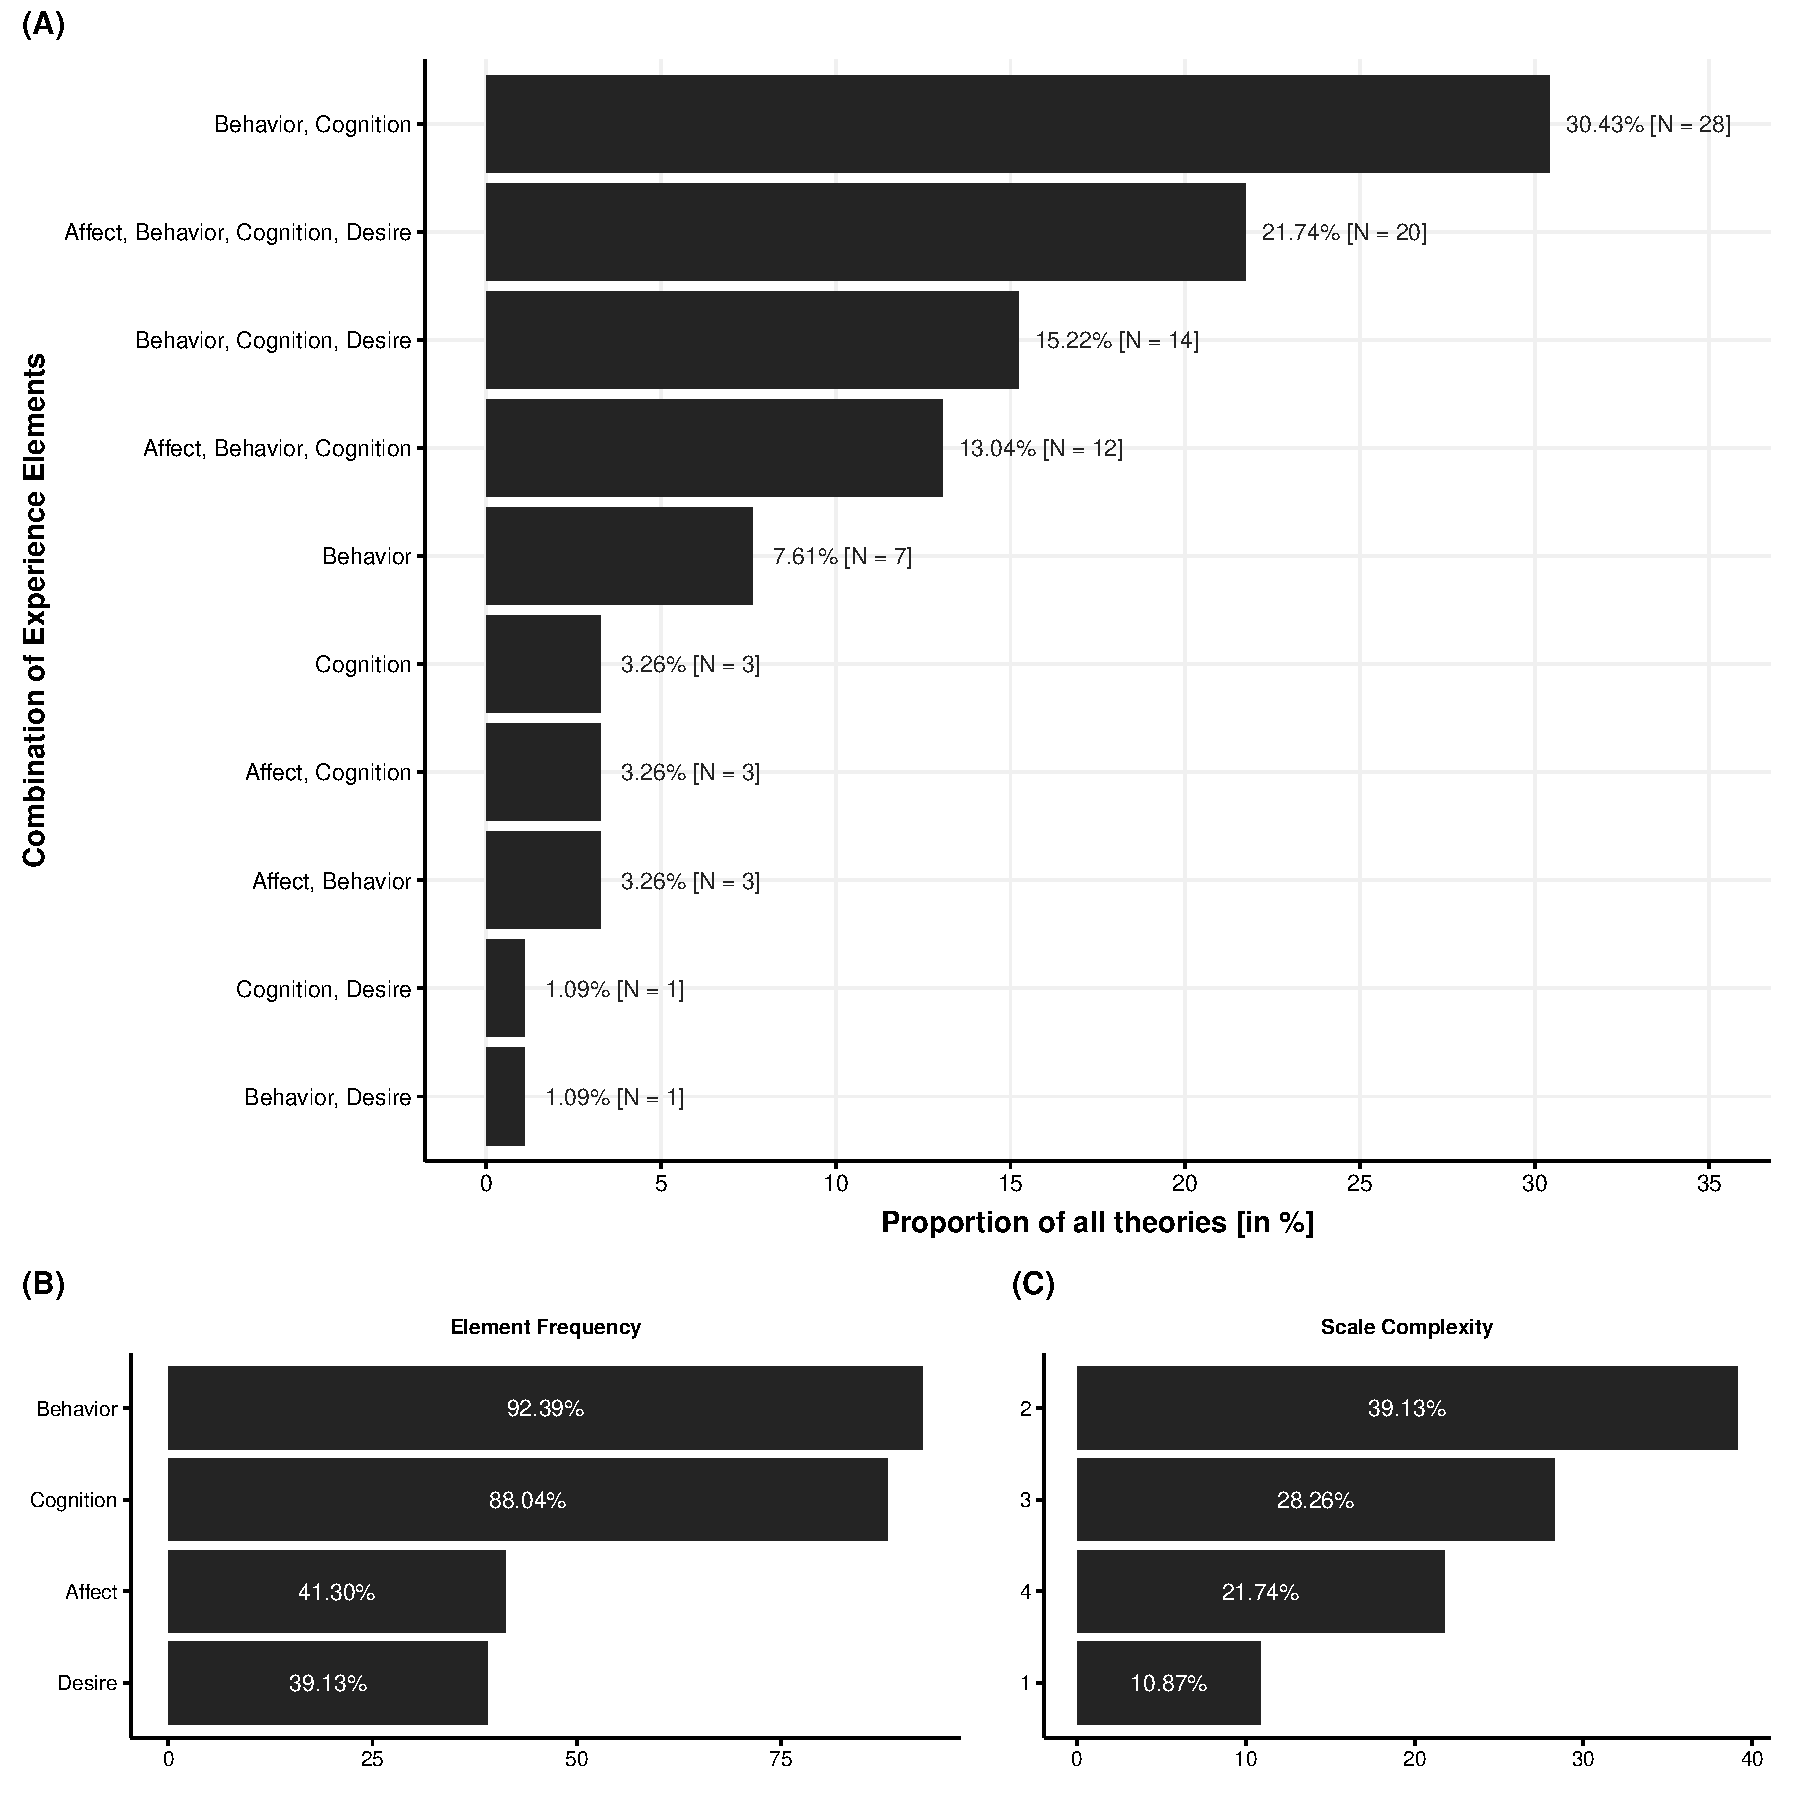
\includegraphics[width=\textwidth]{Figures/TheoriesFreq-1}
\label{fig:ElementsTheories}
\end{figure}

\begin{table}
\begin{minipage}[t][\textheight][t]{\textwidth}

\caption{\label{tab:CombinedCooccurrences}Bivariate Asspociation of Aspects for all Literature Levels.}
\begin{tabular}[t]{lcccc}
\toprule
\multicolumn{1}{c}{Aspect} & Affect & Behavior & Cognition & Desire\\
\midrule
\addlinespace[0.3em]
\multicolumn{5}{l}{\textbf{Theoretical (\textit{N} = 92)}}\\
\hspace{1em}Affect & \textit{N} = 38 & -0.01 & 0.11 & 0.23*\\
\hspace{1em}Behavior & 35 & \textit{N} = 85 & -0.11 & 0.15\\
\hspace{1em}Cognition & 35 & 74 & \textit{N} = 81 & 0.23*\\
\hspace{1em}Desire & 20 & 35 & 35 & \textit{N} = 36\\
\addlinespace[0.3em]
\multicolumn{5}{l}{\textbf{Methodological (\textit{N} = 233)}}\\
\hspace{1em}Affect & \textit{N} = 117 & -0.05 & 0.22*** & 0.22***\\
\hspace{1em}Behavior & 83 & \textit{N} = 170 & -0.08 & -0.10\\
\hspace{1em}Cognition & 111 & 146 & \textit{N} = 204 & 0.16*\\
\hspace{1em}Desire & 46 & 45 & 65 & \textit{N} = 68\\
\addlinespace[0.3em]
\multicolumn{5}{l}{\textbf{Empirical (\textit{N} = 526)}}\\
\hspace{1em}Affect & \textit{N} = 259 & 0.03 & 0.29*** & 0.09*\\
\hspace{1em}Behavior & 210 & \textit{N} = 421 & -0.10* & -0.02\\
\hspace{1em}Cognition & 241 & 336 & \textit{N} = 430 & 0.09\\
\hspace{1em}Desire & 57 & 76 & 86 & \textit{N} = 97\\
\bottomrule
\multicolumn{5}{l}{\rule{0pt}{1em}\textit{Note: }}\\
\multicolumn{5}{l}{\rule{0pt}{1em}Diagonal: Times aspect occurred;}\\
\multicolumn{5}{l}{\rule{0pt}{1em}Upper triangle: Phi association;}\\
\multicolumn{5}{l}{\rule{0pt}{1em}Lower triangle: Times aspects co-occurred.}\\
\end{tabular}
\end{minipage}
\end{table}


\subsection{Psychometric Literature}

Based on the systematic scoping review and its coding, the first
empirical dataset we assess is a database of scale validations. We bring
together the scales suggested in previous reviews as well as validation
studies we identified in our own review. Throughout our literature
review, we found five major works that reviewed the measurement of
acculturation
\citep{Celenk2011, Maestas2000, Matsudaira2006, Wallace2010, Zane2004}.
After removal of duplicate scales, we added any scale validation that
was present in our own systematic scoping review but not included in the
previous reviews. For each measure, we extracted the full item list as
well as the item scoring prior to coding. A comprehensive and
interactive database of the scales, with all available items, reference-
and publication information, as well as our experience elements and
-context coding is available in Supplemental Material D (also see
\fgrref{fig:DirectoryScreen} for an illustration).

\begin{figure}[ht!]
  \centering
  \caption{Screenshot of the \textit{Acculturation Scale Directory}. Top: Main table of the included acculturation scales as well as the filter interface. Bottom: Detailed view of selected scale with item, response, sample, and life domain information. A full description of the directory is available in Supplemental Material D and the directory is available at: \href{https://acculturation-review.shinyapps.io/scale-directory/}{https://acculturation-review.shinyapps.io/scale-directory/}.}
  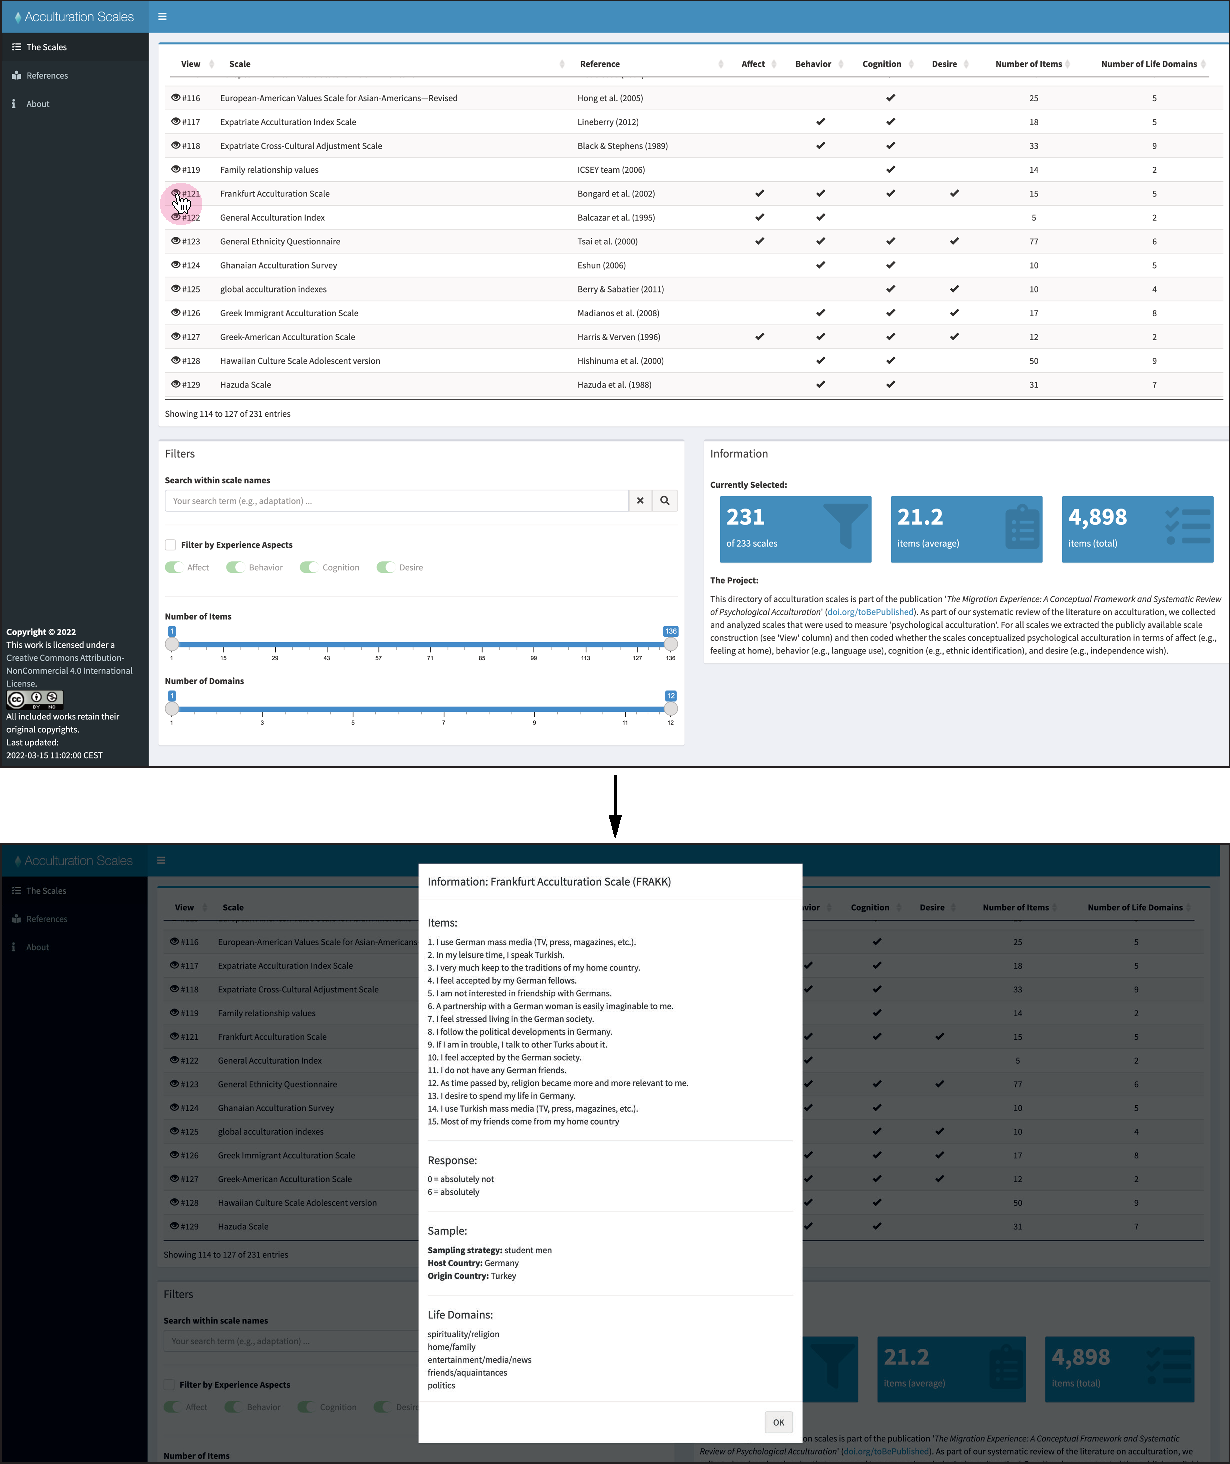
\includegraphics[width=\textwidth]{Figures/AcculturationDIrectoryScreenshot.pdf}
  \label{fig:DirectoryScreen}
\end{figure}

\subsubsection{Methods}  
\paragraph{Dataset}

After duplicate removal, these five reviews collected a total of 97
scales. From our own review, we added 159 additional validation studies
(total of 256 unique scales). Of these scales, we ultimately had to
exclude 23, because they were either not accessible or did not fit the
topic of our review (see \tblref{tab:ExclusionsCombined}). About a
quarter of scales (24.22\%) included majority group members in their
validation studies. The earliest included validation was from 1948 with
a majority of scales being validated around the turn of the
21\textsuperscript{st} century and the most recent included validation
study was published in 2020.

\paragraph{Experience Aspects}

We extracted data on the experience aspects by primarily focusing on the
measured concepts and their operationalizations (also see
\tblref{tab:AspectExamples}). For each article, we retrieved the items
used and coded whether the measure included references to affects,
behaviors, cognitions, and desires. Because this concerned the most
central aspect of our framework, each manuscript was double-coded and
inconsistent codes were resolved after discussion (all inter-rater
agreements were 97.85\% or above and all Cohen's \(\varkappa\)s were
above 0.95, \(\varkappa_{pooled}\) = 0.96; for full inter-rater
reliability see Supplemental Material C).

At this stage, we also noted if scales or items measured concepts that
relate to multiple experience aspects. As an example, a single item
asking about `satisfaction with the new life' might include emotional
and cognitive elements. In this case, we code the manuscript as
measuring both emotions and cognitions, and noted that these elements
are not measured independently. We also noted if the measures do not
consider an individual's experiences, such as reporting migration status
or length of residency.

\paragraph{Process}

To extract an indicator of whether the scales were aimed at
psychological acculturation as a process or an outcome, we collected
information on assessed migration times (e.g., pre-migration,
post-migration) and the the validation type (e.g., cross-sectional,
longitudinal).

\subsubsection{Results}

\paragraph{ABCD prevalence.}

With our main aim of examining the experience structure within the
scales, we examined whether scales included a specific experience
element but also examined the used elements in their complex
combinations. In terms of general inclusion of elements, most studies
included a measure of cognition (87.55\%) and behavior (72.53\%),
whereas only roughly half the studies included a measure of affect
(50.21\%) and only a fourth of the scales included a measure of desires
(29.18\%). However, only a minority of scales included only a single
aspect. There were only 18 scales that exclusively relied on cognitions
(7.73\%) and 21 scales that measured only behaviors (9.01\%). Yet,
inversely, there were also only 35 scales that measured all four aspects
(15.02\%). Most studies measured two (38.63\%) or three (27.9\%)
aspects. A majority of scales either measured behavioral and cognitive
aspects (23.61\%) or behavioral, cognitive, and affective elements
(19.31\%; also see \fgrref{fig:ElementsScales} and
\tblref{tab:CombinedCooccurrences}).

\paragraph{ABCD composition.}

Looking at the number of aspects measured together we also see
substantial differences in what kind of scales include a certain aspect.
Scales that included cognitions also measured an average of 1.57 others
aspects (\textit{SD} = 0.77), scales measuring behavior, on average,
also included 1.62 other aspects (\textit{SD} = 0.77). Scales measuring
affect or desire measures included substantially more other aspects.
Scales that included affect measures also included 2.04 other aspects
(\textit{SD} = 0.61) and scales measuring desires even measured an
average of 2.31 other aspects per scale (\textit{SD} = 0.66; also see
\fgrref{fig:LiteratureComparison}). Thus, most scales measure multiple
dimensions (\textit{M} = 2.39, \textit{SD} = 0.91), yet they focus on
external accessible aspects of psychological acculturation (i.e.,
behavior and cognition), less of what is considered `internal' or
`subjective' (i.e., affect and desires). And if affect or desire
elements are considered, they often only occur in scales that already
include a higher number of other aspects. This is further underscored by
the observation that there were only 3 scales that exclusively measured
emotional acculturation and not a single scale that exclusively focused
on motivational acculturation (while this was the case for both
cognitions and behaviors).

\begin{figure}[h]
\centering
\caption{Psychological Acculturation Aspects within the Psychometric Literature. (A) Bar graph showing the common combinations of the affect, behavior, cognition, desire experience aspects. (B) Bar graph showing the prevalence of each experience aspect within the literature. (C) Bar graph showing how many experience aspects were considered together.}
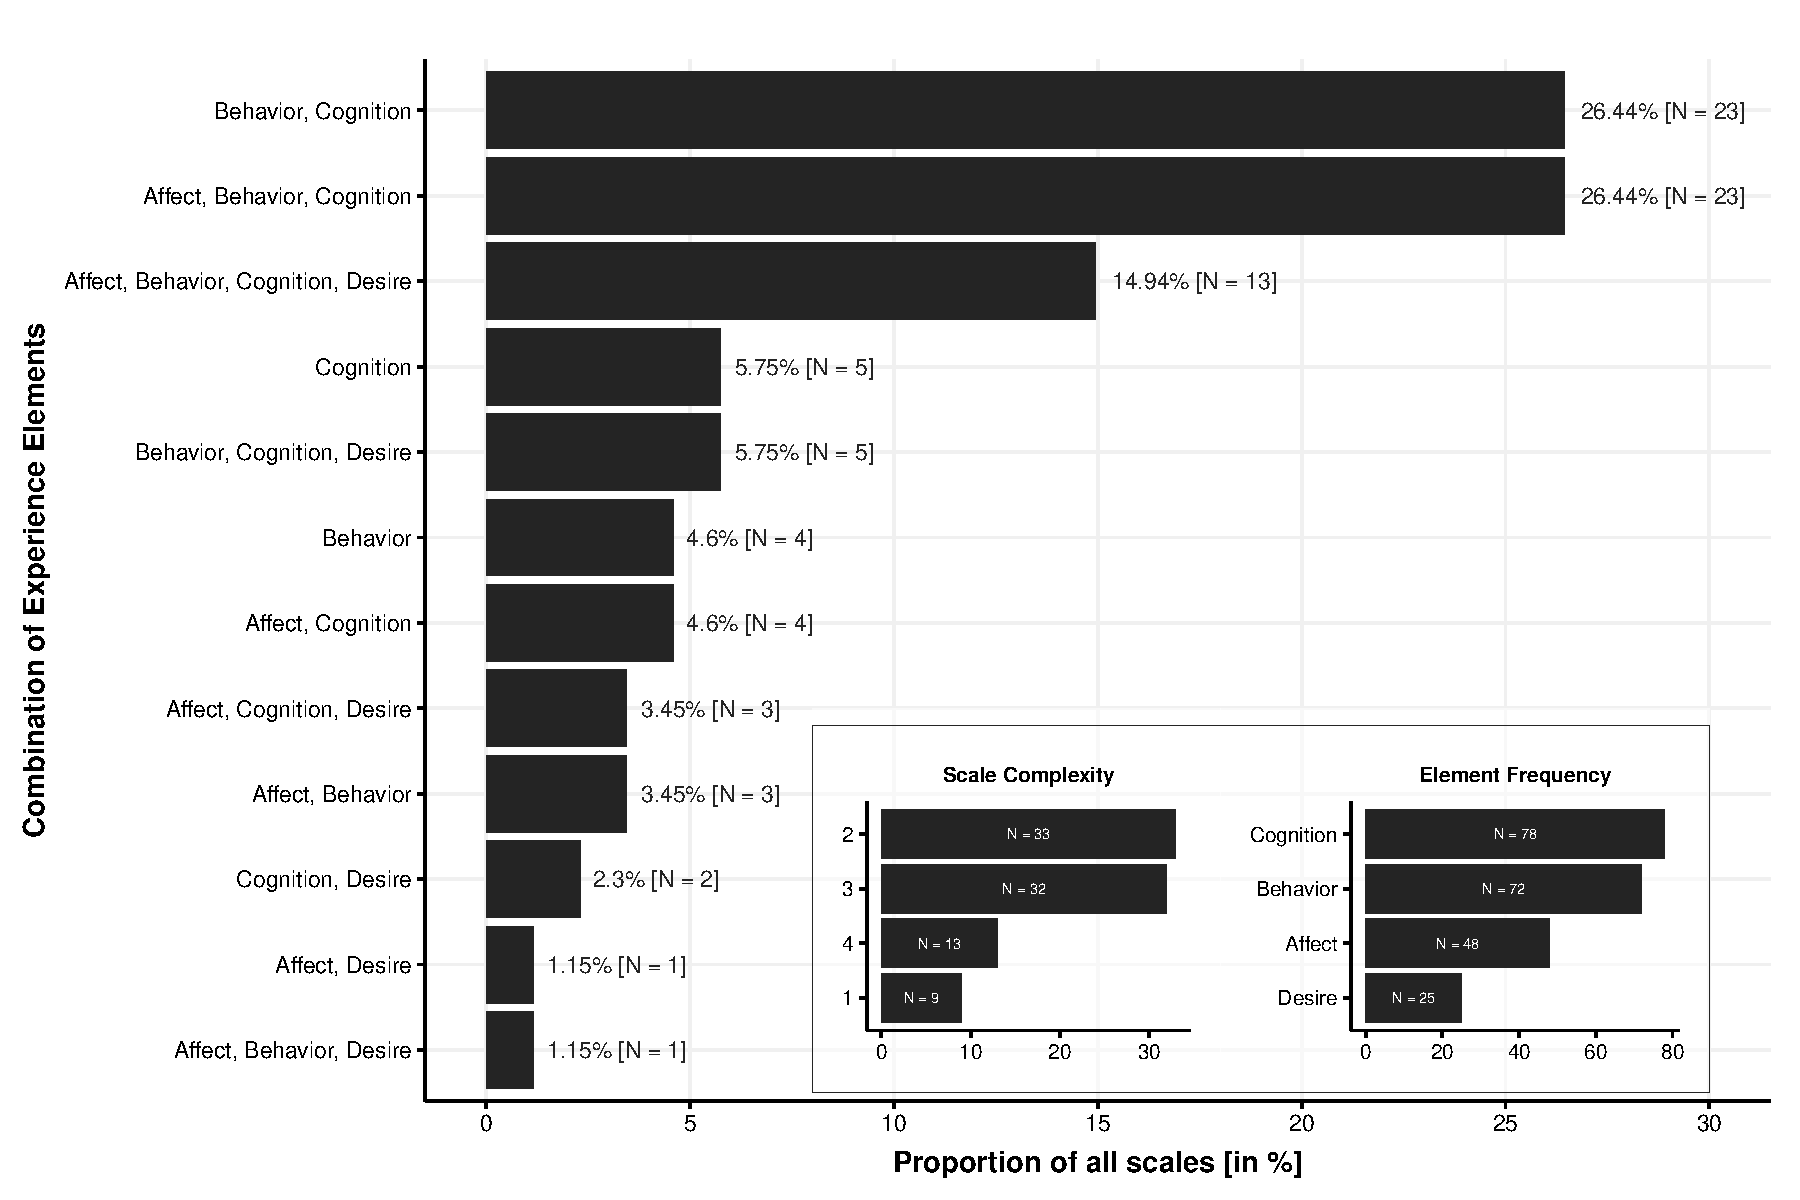
\includegraphics[width=\textwidth]{Figures/ABCDFreq-1}
\label{fig:ElementsScales}
\end{figure}

\paragraph{Process.}

To assess the process focus of the scales we also assessed the migration
time the scale validators considered. Except for a single scale that was
validated for potential migrants, all scales were validated using
cross-sectional data after the migrant arrived in the settlement
society. This is in line with observations by previous reviews of the
field \citep[e.g.,][]{Brown2011}.

\paragraph{Content.}

While a discussion of all the topics addressed by the included scales
lies beyond the scope of this study, we would like to describe some of
the larger patterns authors have focused on. To that aim, we offer
illustrations of the patterns we observed during the reading,
extraction, and coding of the acculturation scales. We additionally, ran
a machine learning topic modeling procedure on the items of the scales
to identify content topics.

A first key observation is that there was considerable diversity between
the scales in how many experience aspects and topics were addressed.
That might not generally be surprising, considering that the scales had
between 1 and 136 items, and included between 1 and 12 life domains (see
Supplemental Material E). Additionally, scales were also either more
focused on a specific aspect
\citep[e.g., `Asian Value Scale';][]{Kim1999, Kim2004a} or aimed to
capture acculturation more broadly
\citep[e.g., `Asian American Multidimensional Acculturation Scale'][]{GimChung2004}.
Another trend that we observed was a separation between a factual and
counter-factual acculturation
\citep[e.g., real vs. ideal,][]{Navas2005, Navas2007, BenetMartinez2006}.
Additionally, while a large number of scales separately assessed ABCDs
as they related to the dominant culture and the heritage culture, we saw
a trend towards explicitly asking about different life domains
\citep[e.g., family, work, media;][also see Supplemental Material E]{Kim2010a, Arends-Toth2007, Mancini2014}.

When considering the content of the aspects that were included across
acculturation scales, the topic modeling analysis offers a number of key
insights that mostly align with our reading of the literature. For the
topic modeling of the acculturation scales, we particularly used the
scale items in a Latent Dirichlet Allocation (LDA) analysis, an
unsupervised machine learning method common within the natural language
processing literature. The analysis essentially extracts sets of terms
that tended to occur together, assuming that scales that measure a
specific topic have more words that relate to the topic than scales that
measure other topics
\citep[we followed the procedures outlined by][for a full methodological detail see Supplemental Material C]{Schweinberger2022}.

While we had earlier described that many scales included a measurement
of behavioral acculturation, the topic modeling showed that one of the
main topics across the scales was language use. This included questions
about listening to, reading, and speaking the dominant local language.
While there are a few (sub-)scales specifically targeting language use
as a conceptualization of acculturation
\citep[e.g.,][]{Deyo1985, ICSEYteam2006}, most scales used language as
only one of multiple experience aspects. Moreover, the assessment of
behavioral language use (and the more cognitive language proficiency)
often differentiated between language used at home and outside the home.
Similarly, some language assessments were distinguishing between the
languages used in different life areas
\citep[ e.g., media consumption, among friends, at work][for more information see Supplemental Material C]{Birman2002}.
Other behavioral measurements of acculturation included the
participation in and celebration of traditions and customs
\citep[e.g.,][]{Rezentes1993, Wilson2013, Cortes1994}, clothing
\citep[e.g.,][]{Ghuman2000}, food \citep[e.g.,][]{Schaefer2009}, and
political participation \citep[e.g.,][]{Jeong2016, Uslaner2005}. One
pattern that the topic modeling procedure highlighted was that food
related questions were often found in scales targeting the adaptation of
Asian migrants (in particular, Vietnamese, Indian, and Korean
acculturation scales).

Among the cognitive conceptualizations of acculturation, one key topic
that we saw both in the LDA and in our own review process is a strong
focus on ethnic identification and cultural identity ratings
\citep[e.g.,][]{Jadalla2015, Mchitarjan2015}. Other important topics
were belief- \citep[e.g.,][]{Klonoff2000} and value endorsement
\citep[e.g.,][]{Kim2010a, Wolfe2001, Duarte2020}, as well as preferences
\citep[e.g.,][]{BenetMartinez2006, Tull2003}.

Among the affective acculturation measurements an important distinction
was the separation by valence, often either assessing joy and happy
\citep[e.g.,][]{Phinney1992, Cuellar1995a}, or anxiety and loneliness
\citep[e.g.,][]{Shin1999, Perez2019}. A second observation was a
particular focus on self-conscious emotions, such as pride and shame
\citep[e.g.,][]{Tsai2000, Suinn1992}. A third pattern was that most of
the emotional measurements were of social emotions, such as comfort and
discomfort \citep[e.g.,][]{Stephenson2000}, or belonging and
connectedness feelings \citep[e.g.,][]{Kouli2009, Harder2018}.

Most of the motivational acculturation measurements (i.e., desires) were
related to wishes and wants for the future
\citep[e.g.,][]{Mancini2014, Ben-Shalom2003}. However, there was a
smaller subset of scales explicitly addressing specific motives, such as
transition motives \citep[][]{Mchitarjan2015}, motivation for cultural
exploration and maintenance \citep[][]{Recker2017}.

It should be noted that with the psychometric literature we saw a larger
number of instances where items targeted multiple experience aspects
\citep[e.g., enjoyment of wearing traditional clothing,][]{Ozer2016} as
well as the measurement of concepts that included multiple experience
aspects \citep[e.g., satisfaction,][]{Cuellar1995a}.

Finally, there were a few additional patterns that were particularly
hightlighted by the LDA topic modeling. These issues included a focus on
navigating everyday life issues \citep[e.g.,][]{Harder2018}, and
acculturation hassles \citep[e.g.,][]{Vinokurov2002}, as well the
importance of family and generational differences
\citep[e.g.,][]{ICSEYteam2006, Lee2004b}. Similarly, the topics
showcased that the validated scales tended to focus on specific cultural
pairs, such as migrants from the former UDSSR in Israel, or Mexicans and
East Asians in North America (for more information on the migration
context see Supplemental Material E). Please also note that we developed
an interactive scale directory, where users can explore the content of
the included acculturation scales on their own (see Supplemental
Material D).

\subsection{Empirical Literature}

At the most applied level, we assessed the broader empirical studies.
This final database included the largest number of manuscripts and is in
theory the application of the theoretical and psychometric literature.
The search produced a total of 1,629 results to which we added 133
articles through contacts with experts in the field and from referenced
works within the review. After duplicate removal, title--, abstract--,
and full-text screening we coded a total of 526 empirical works (for
exclusion reasons see \tblref{tab:ExclusionsCombined} and for the PRISMA
diagram see \fgrref[ C]{fig:PrismaCombined}).

\subsubsection{Methods}

\paragraph{Dataset}

Of the final works we coded, 452 were journal articles, 68 theses, and 6
book chapters. Most studies presented quantitative data (\textit{N} =
464), mixed methods (\textit{N} = 39), or qualitative data (\textit{N} =
20), while the remaining 3 manuscripts were reviews of empirical data.
Notably, a majority of the empirical investigations did not share common
measures of acculturation --- 391 studies used measures that were
reported a maximum of five times. A considerable majority of papers with
uncommon measures used new or ad-hoc measures of acculturation. Less
than a fifth of studies included local majority group members in the
study (\textit{N} = 77, 14.69\%). Acculturation most frequently was a
predictor variable (\textit{N} = 285, 54.39\%), a dependent variable
(\textit{N} = 148, 28.24\%), or a correlation variable (\textit{N} = 37,
7.06\%) in the empirical works. This pattern was mirrored when looking
at the focus of the papers, where a majority of the papers had
acculturation as their main focus (\textit{N} = 153, 29.48\%), with
other bodies of work focusing on health outcomes (\textit{N} = 163,
31.41\%), or inter-group relations (\textit{N} = 18, 3.47\%) as their
main outcomes. The earliest included study was published in 1948, with a
strong increase of publications after the year 2000, and a peak of
publications in 2012. We provide full descriptions of data extractions
and additional information about the data description in Supplemental
Material C.

\paragraph{Experience Aspects}

Extraction of the used experience aspects mirrored the psychometric
literature assessment and we primarily focused on the measured concepts
and their operationalizations (also see \tblref{tab:AspectExamples}).
The only exception were qualitative studies, which we coded following
the same codebook of the theoretical literature. All aspects were coded
by two independent coders (all inter-rater agreements were 97.91\% or
above and all Cohen's \(\varkappa\)s were above 0.93,
\(\varkappa_{pooled}\) = 0.97; for full inter-rater reliability see
Supplemental Material E) and inconsistencies were resolved after
discussion.

\paragraph{Process}

To assess the static or dynamic conceptualization of the empirical
studies, we again collected information on assessed migration times
(e.g., pre-migration, post-migration) and additionally coded the type of
data collected and analyzed (e.g., cross-sectional, longitudinal data
and data analysis).

\paragraph{Field of Publication}

For the broader empirical literature, we also collected additional data
on the field the studies were published in. To that end, we merged the
`Scimago Journal Ranking Database' \citep{SCImago2020} with our
database. For all available journal articles, we added information on
key journal metrics (incl.~H index, impact factor, and data on the field
and audiences). This also meant that dissertations, book chapters, and
books were excluded from this analysis because data on their publishers
is not readily available or unreliable. Additionally, 19 journals were
not included in the Scimago database (because they do not have an ISSN
identifier or were discontinued before 1996, see Online Appendix B for
the missing journals). We ultimately had journal metrics for 425
empirical articles.

To summarize the journal data we then classified the journal fields into
super-ordinate discipline codes. These discipline codes are based in
part on the U.S. Department of Education's subject classifications
\citep[i.e., CIP,][]{InstituteofEducationSciences2020}, the U.K.
academic coding system
\citep[JACS 3.0,][]{HigherEducationStatisticsAgency2013}, the Australian
and New Zealand Standard Research Classification
\citep[ANZSRC 2020,][]{AustralianBureauofStatistics2020}, as well as the
Fields of Knowledge project \citep{ThingsmadeThinkable2014}. We
ultimately classified each journal into one of four mutually exclusive
disciplines (`psychology': \textit{N} = 122, `multidisciplinary':
\textit{N} = 102, `medicine, nursing, and health': \textit{N} = 144, and
`social sciences (miscellaneous)': \textit{N} = 45. For a full
discussion of the classifications see Online Supplemental Material C).

\subsubsection{Results}

We assessed the role of experience aspects in the measurement and then
compared differences between fields.

\paragraph{ABCD prevalence.}

In terms of the overall frequencies of experience elements, the broader
empirical data mirrored that of the psychometric literature. Most
studies included a measure of cognition (81.75\%) and behavior
(80.23\%), whereas only about half of all studies included a measure of
affect (49.05\%) and less than a fifth of the studies included a measure
of desires (18.63\%). Yet, only 126 studies focused on a single
experience aspect (\(N_{behavior\ only}\) = 73, \(N_{cognition\ only}\)
= 47, \(N_{emotion\ only}\) = 6). Similarly, only 46 papers included
measures of all four experience aspects (8.75\%). Most studies measured
three (36.12\%) or two aspects (31.18\%; \textit{M} = 2.30, \textit{SD}
= 0.86). Different from the scale validations, within the broader
empirical works, most works included measures of emotions, behaviors,
and cognitions (\textit{N} = 158, 30.04\%), with a further substantial
number of articles measuring behaviors and cognitions (\textit{N} = 107,
20.34\%. Also see \fgrref{fig:EmpPlotFreq-1} and
\tblref{tab:CombinedCooccurrences}).

\paragraph{ABCD composition.}

Looking at the number of aspects measured together we again see
substantial differences in what kind of scales include the individual
aspects. Scales that included cognitions measured an average of 1.54
other aspects (\textit{SD} = 0.68), scales measuring behavior, on
average, measured 1.48 other aspects (\textit{SD} = 0.82), while scales
that included affect measured an average of 1.97 other experience
aspects (\textit{SD} = 0.43) and scales measuring desires even measured
an average of 2.27 other experience aspects (\textit{SD} = 0.61; also
see \fgrref{fig:LiteratureComparison}). Thus, not a single study
measured only motivational acculturation (i.e., desires), and measures
of desires remained mostly limited to scales that were already measuring
many of the other experience aspects. The results exacerbate the pattern
found in the scale validations, complex measures and conceptions of
acculturation are seen infrequently and external aspects of cognition
and behavior remain the focus of most studies.

\begin{figure}[h]
\centering
\caption{Psychological Acculturation Aspects within the Empirical Literature. (A) Bar graph showing the common combinations of the affect, behavior, cognition, desire experience aspects. (B) Bar graph showing the prevalence of each experience aspect within the literature. (C) Bar graph showing how many experience aspects were considered together.}
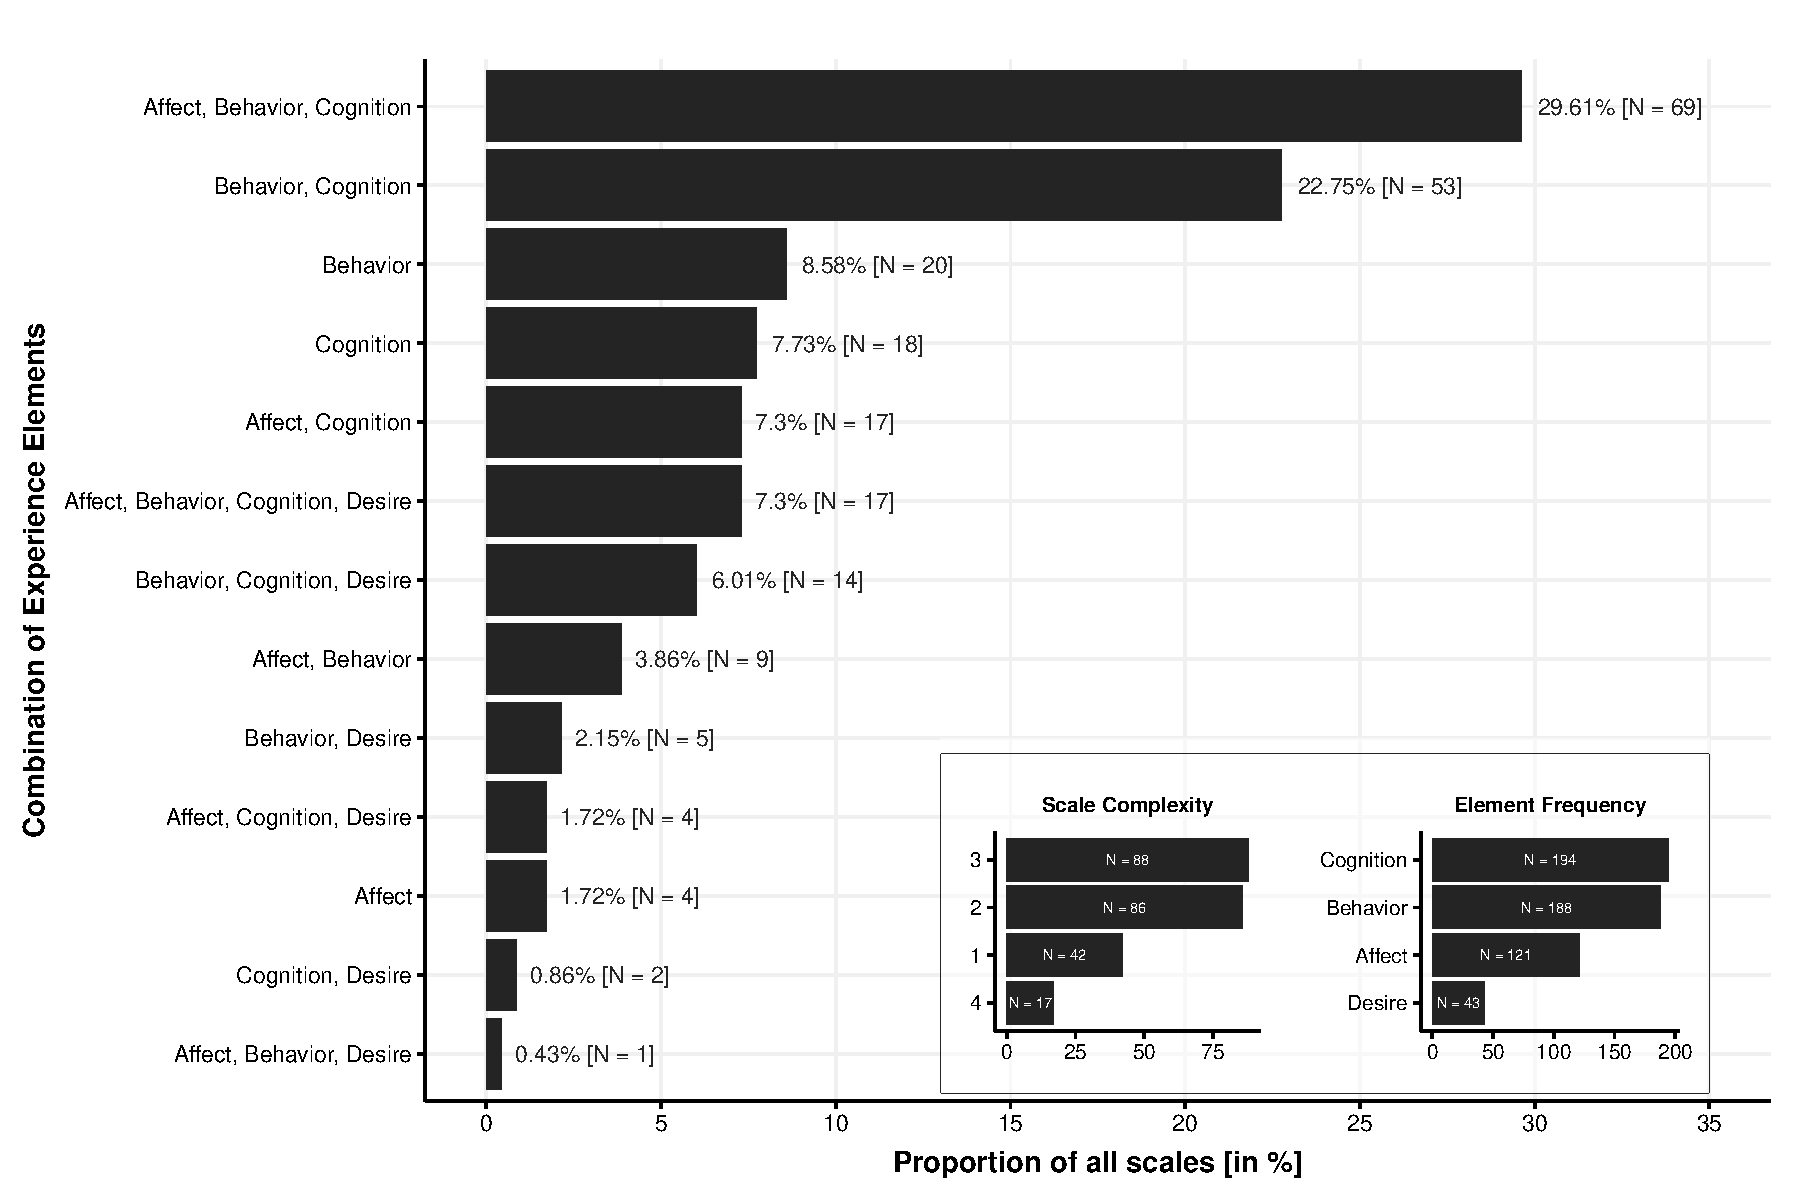
\includegraphics[width=\textwidth]{Figures/EmpPlotFreq-1}
\label{fig:EmpPlotFreq-1}
\end{figure}

\paragraph{Process.}

To assess the process focus of the broader empirical works, we again
assessed when in the migration process the data was collected and we
additionally assessed the type analysis done by the authors. We found
that 512 studies (97.71\%) collected data after the arrival of the
migrant in the new society. Two studies targeted potential migrants and
10 studies collected data prior to and following the migration event.
Moreover, only 25 studies included longitudinal data analyses of
psychological acculturation (4.79\%). This observation again underscores
the arguments that the acculturation literature has thus far failed to
provide data that meaningfully captures migration as a process
\citep[e.g.,][]{Brown2011, Ward2019}.

\paragraph{Content.}

When considering the content of the empirical conceptualizations of
psychological acculturation, the content largely mirrors that of the
psychometric literature, whenever authors used validated acculturation
scales. However, there were a few conceptualizations that were favored
in empirical practice. One such focus has been that specific
acculturation scales were used more frequently. These favored scales
including the `Vancouver Index of Acculturation' \citep[][]{Ryder2000},
the `Language, Identity, and Behavioral Acculturation Scale',
`Stephenson Multigroup Acculturation Scale' \citep[][]{Stephenson2000},
as well as scales focusing on Hispanic migrants
\citep[][]{Cuellar1995a, Marin1987, Marin1987}.

Another major pattern within the conceptualizations of applied empirical
works has been the use of modified, abridged, or shortened versions of
established scales \citep[e.g.,][]{Green2014,Im2009}. These scales often
used a subset of questions from the validated scales, for example by
choosing a specific aspect only (e.g., media consumption). This is
different from the use of `adapted' scales, where authors usually only
replaced the name of the dominant and non-dominant cultural groups to
adapt the scale to their context.

An even more extreme version of this pattern has been the observation
that a sizable number of empirical studies has used non-validated
scales. These measurements were often short (i.e., 1-3 items) and lacked
psychometric validation. Common uses were single items on language use,
employment status, or cultural identification. It should be noted that
for many of these studies acculturation was not a key concept of
interest, but rather a covariate or partial outcome variable (for more
information on these conceptualizations see Supplemental Material C).

\paragraph{Comparison publication fields.}

To further assess the comparative utility of the experience framework,
we then assessed differences of experience aspects between academic
fields. For the full results, including differences in the methods, and
publication types as well as contextual differences in terms of sampling
procedures, situational domains, analyses, and cultural contexts see
Supplemental Material C.

We first assessed the references to affect, behavior, cognition, and
desires separately, for each of the disciplines. We find that for all
fields desires (12.5-28.69\% of all measures in the field) and emotions
(35.56-62.3\%) are the least frequently measured elements and medical
journals measure them the least frequently (in proportional terms).
Looking at the common cognitive and behavioral elements the proportions
diverge between the fields. While the multidisciplinary field measured
behaviors (76.47\%) and cognition (82.35\%) almost equally often, in the
medical and general social science journals behaviors were measured
considerably more often than cognitions (\(Behavior_{SoSci}\) = 86.67\%
\textgreater{} \(Cognition_{SoSci}\) = 68.89\%; \(Behavior_{Med}\) =
89.58\% \textgreater{} \(Cognition_{Med}\) = 69.44\%). Inversely, in the
psychological journals cognitions (90.98\%) were measured more often
than behaviors (68.03\%; also see \fgrref[A and B]{fig:FieldPlotFreq}.

When looking at differences in how many different experience aspects
were measured together and patterns within these aspect-combinations,
differences between the fields become increasingly evident (also see
\fgrref[A and C]{fig:FieldPlotFreq}). While `affect, behavior, and
cognition' and `behavior, and cognition' measures are common
combinations across all fields, fewer experience aspects and less
variation were considered in the medical and social science fields.
There were statistically significant mean differences between the fields
in terms of how many experience aspects were considered (parametric:
\textit{F}(3, 409) = 5.02, \textit{p} = 0.002, non-parametric:
\textit{Kruskal-Wallis} \(\chi^{2}\) = 15.01, \textit{df} = 3,
\textit{p} = 0.002, \(\eta_{p}^{2}\) = 0.04, 95\%CI{[}0.01, 1{]}).
Looking at the mean differences in more detail, empirical works
published in psychological journals had significantly higher average
aspect counts (\textit{M} = 2.5, \textit{SD} = 0.83) than the medical
(\textit{M} = 2.1, \textit{SD} = 0.86) and the general social science
journals (\textit{M} = 2.04, \textit{SD} = 0.73; also see
\fgrref{fig:FieldPlotComplexityAverage}). The broader patterns described
here thus point to heterogeneity between fields and show that different
fields diverge in the number and types of acculturation aspects they
tend to consider.

\begin{figure}[h]
\centering
\caption{Scale Complexity and their proportional occurences per field. Stacked bar graphs showing how many experience aspects were measured in each academic field. Holm corrected p-values of the mean differences between academic fields displayed above the chart.}
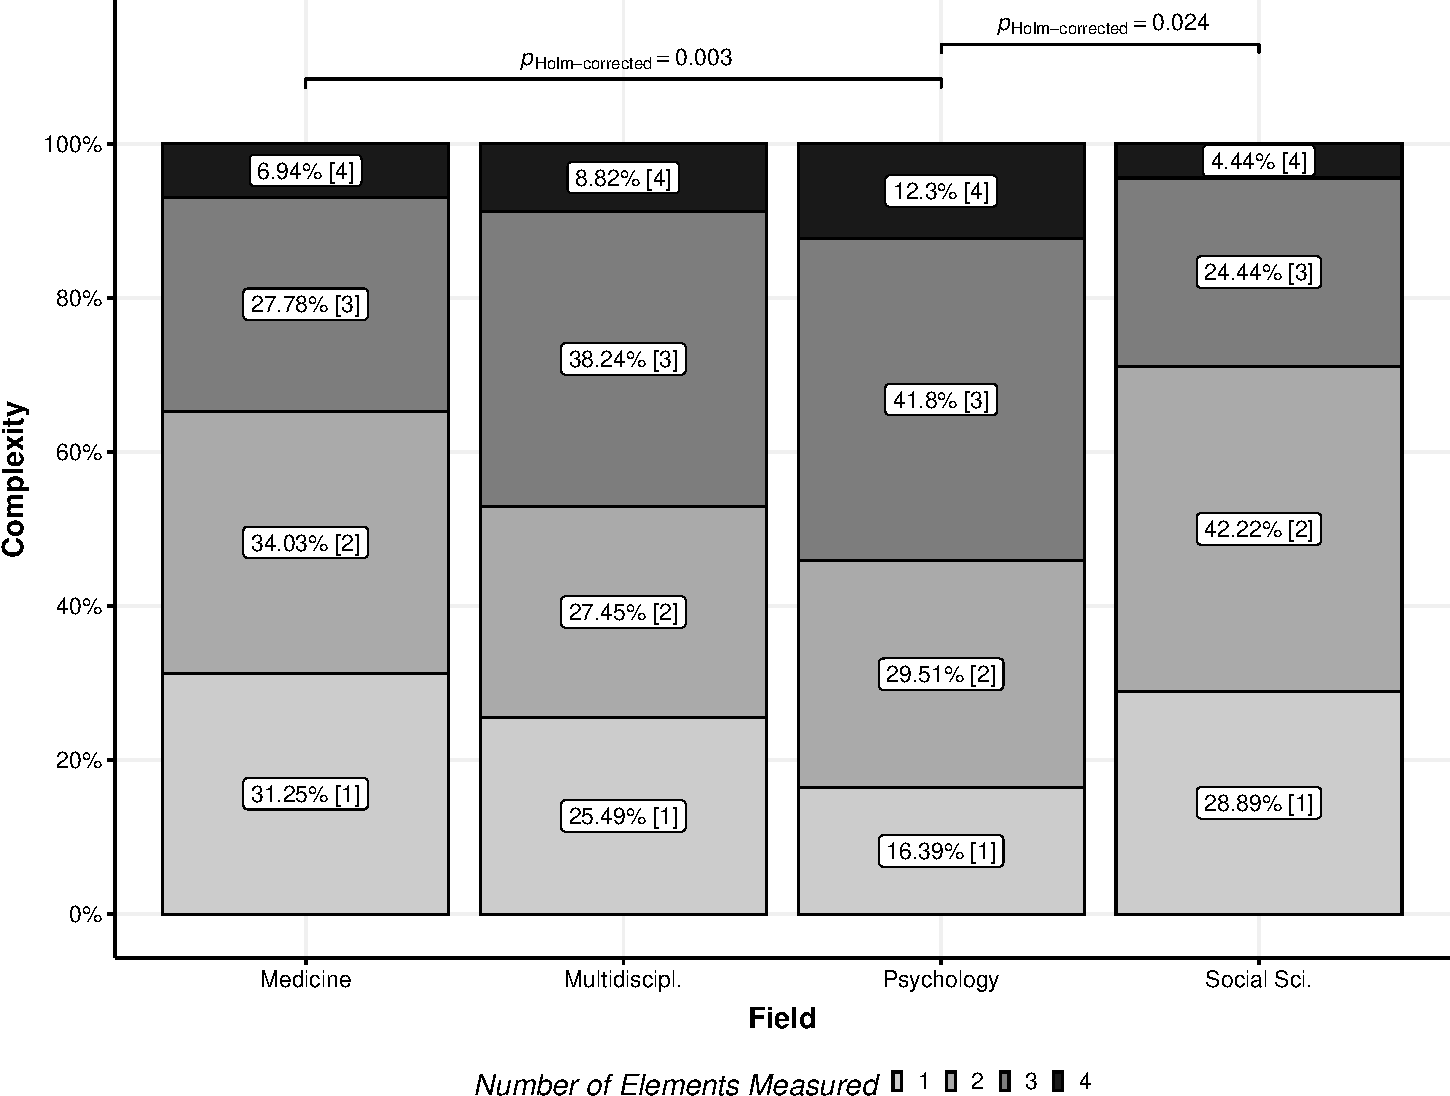
\includegraphics[width=\textwidth]{Figures/FieldPlotComplexityAverage-1}
\label{fig:FieldPlotComplexityAverage}
\end{figure}

\begin{figure}[h]
\centering
\caption{Psychological Acculturation Aspects across different academic fields. (A) Bar graph showing the common combinations of the affect, behavior, cognition, desire experience aspects for each field. (B) Bar graph showing the prevalence of each experience aspect by academic field. (C) Bar graph showing how many experience aspects were considered together in each acdemic field.}
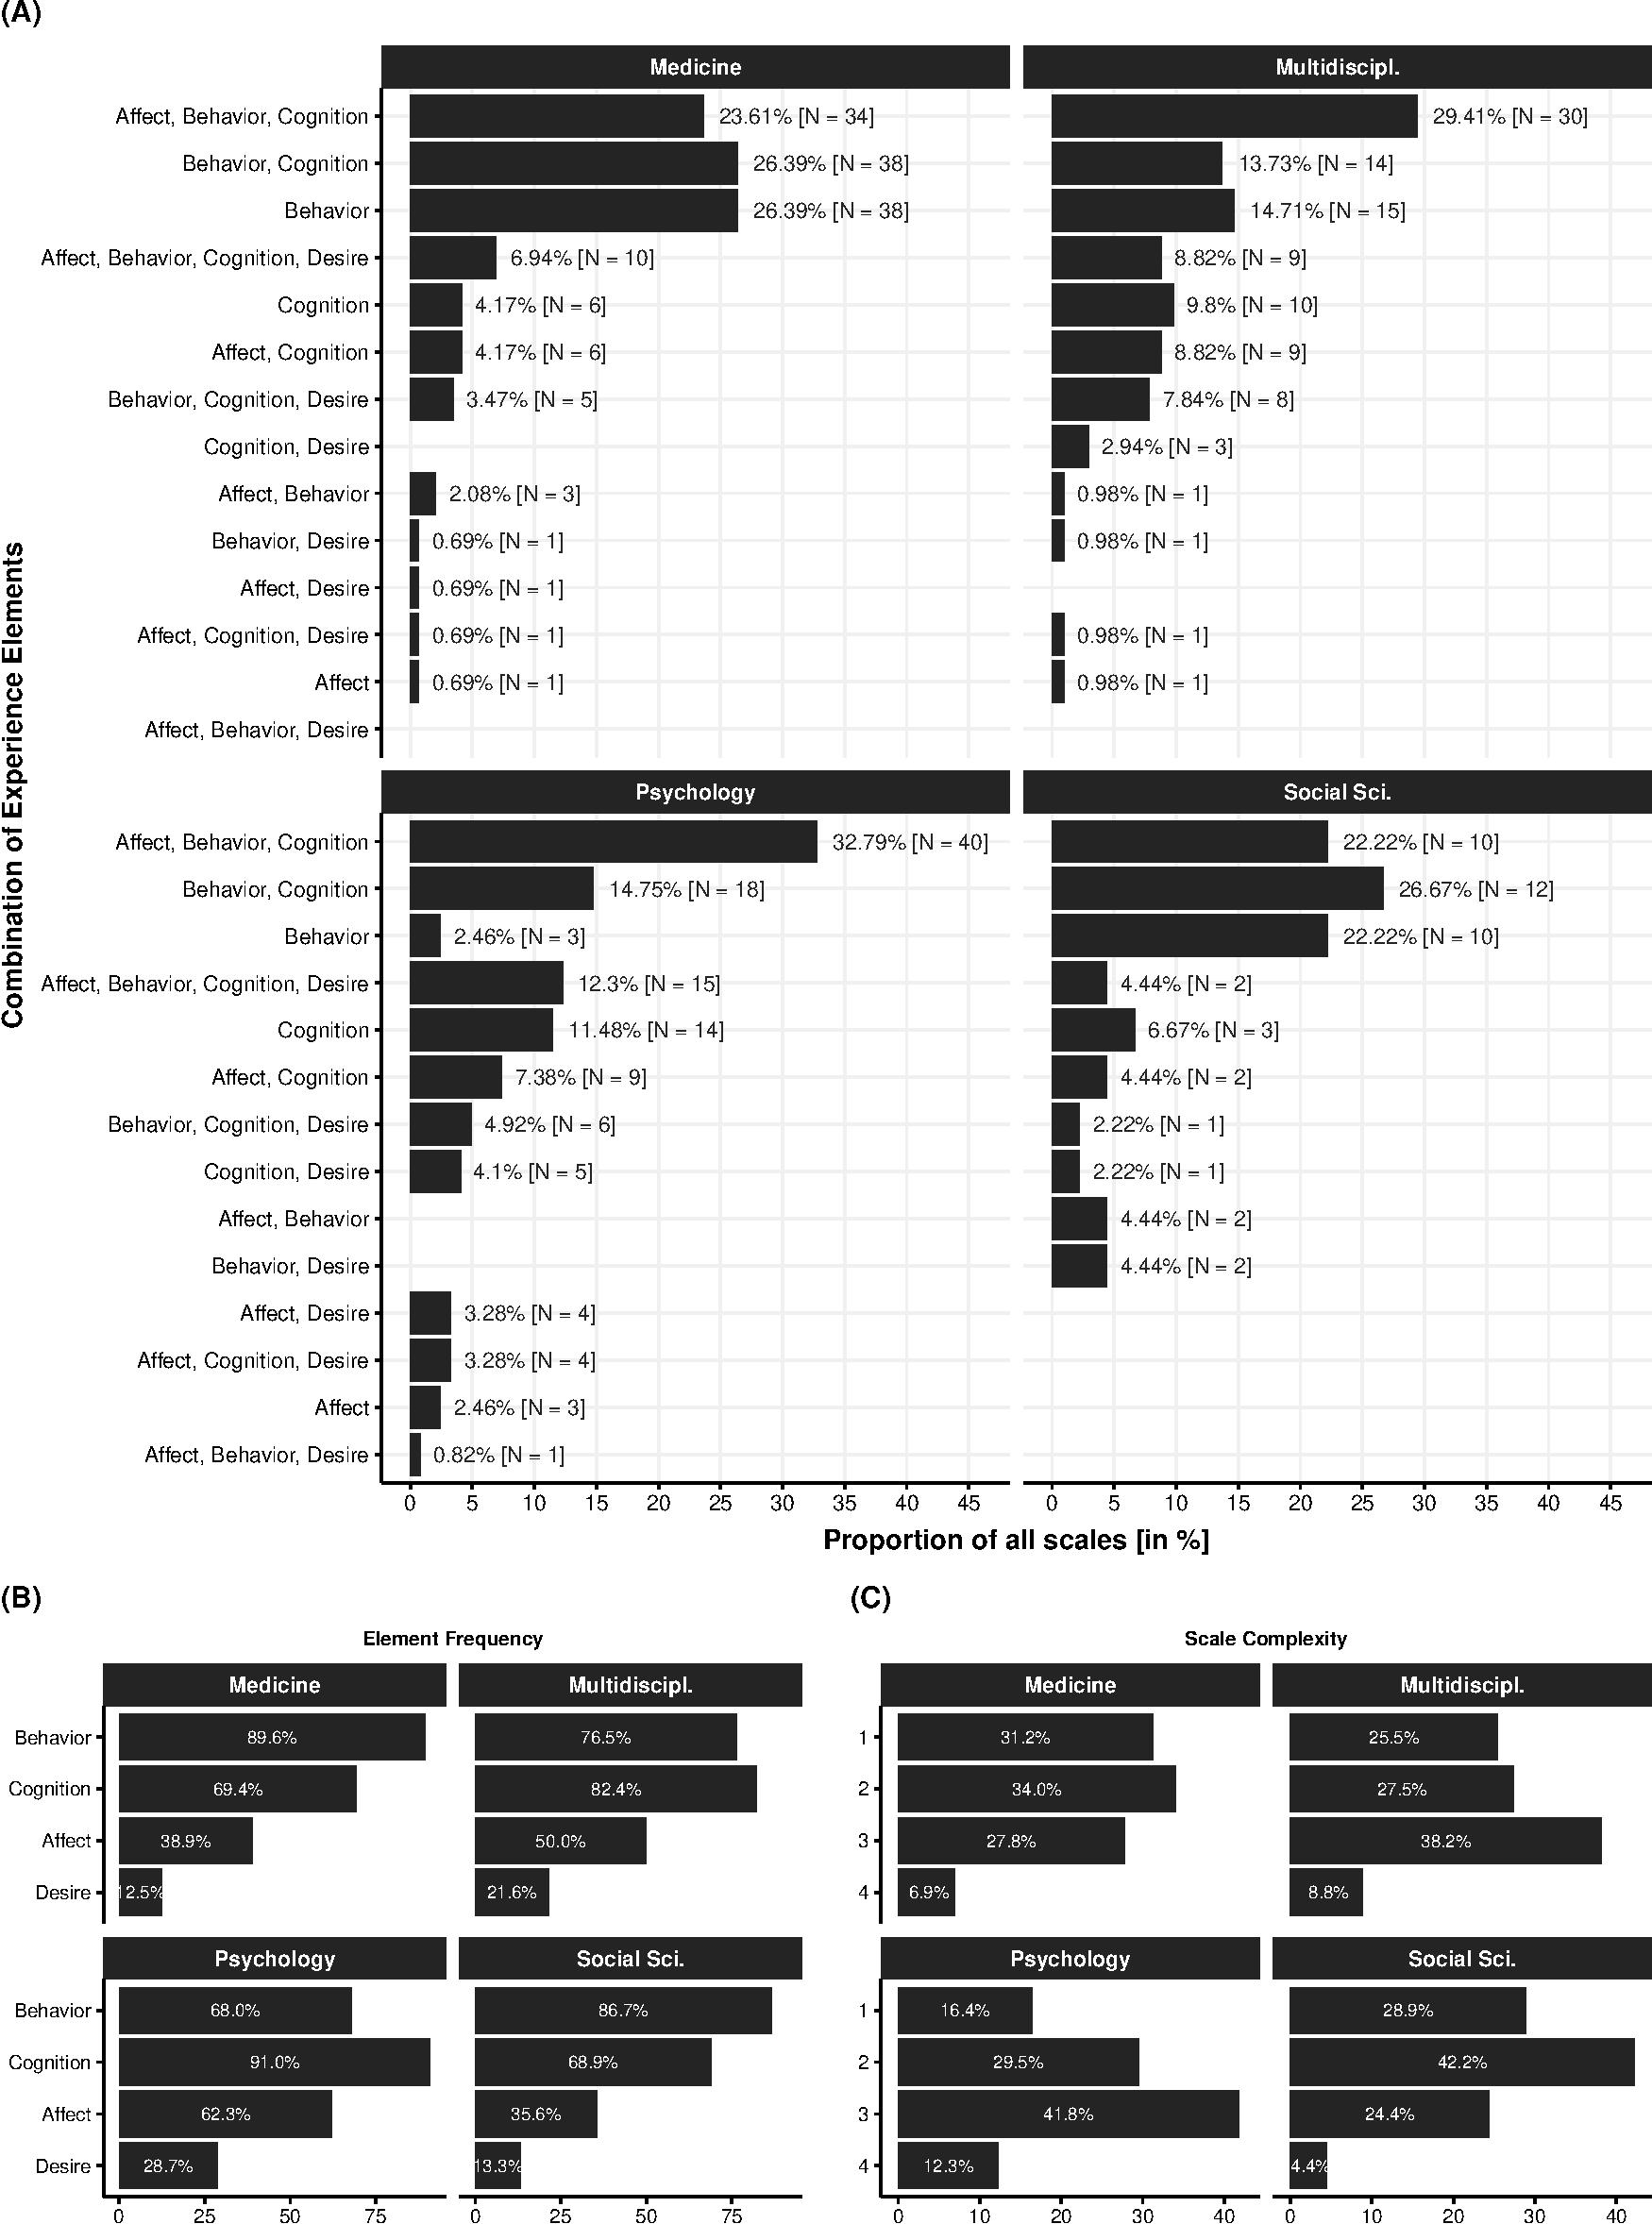
\includegraphics[width=\textwidth]{Figures/FieldPlotFreq-1}
\label{fig:FieldPlotFreq}
\end{figure}

\subsection{Comparing Literature Levels}

As a final step we aim to compare the three levels of literature we have
reviewed (i.e., theoretical-psychometric-empirical). We find that all
three bodies of literature focus more readily on the more external
aspects of behaviors and cognitions, and less on more internal affects
and desires. However, we also see that desires (i.e., motivations) play
a more prominent role in the theoretical literature and interest
decreases with more applied research (also see
\fgrref[A]{fig:LiteratureComparison}). Looking at the combinations of
different experience aspects, we find that across all three bodies of
literature a combination of two or three aspects is most common (often
including behaviors or cognitions). However, we also find that single
aspect conceptualizations are substantially more common in the more
applied empirical works, whereas conceptualizations that include all
four experience aspects are substantially more common in the more
abstract theoretical literature (also see
\fgrref[B]{fig:LiteratureComparison}). Yet, we also see that the most
undervalued aspects often are considered in works that have already
included a larger number of other aspects (also see
\fgrref[C]{fig:LiteratureComparison}).

\begin{figure}[h]
\centering
\caption{Literature Levels: (A) Bar graph of the experience aspect frequencies for theoretical, psychometric, and broader empirical literature. (B) Bar graph of the number of experience aspects used for theoretical, psychometric, and broader empirical literature. (C) Average number of additional aspects included when the aspect was considered for theoretical, psychometric, and broader empirical literature [Mean ± 95\%CI].}
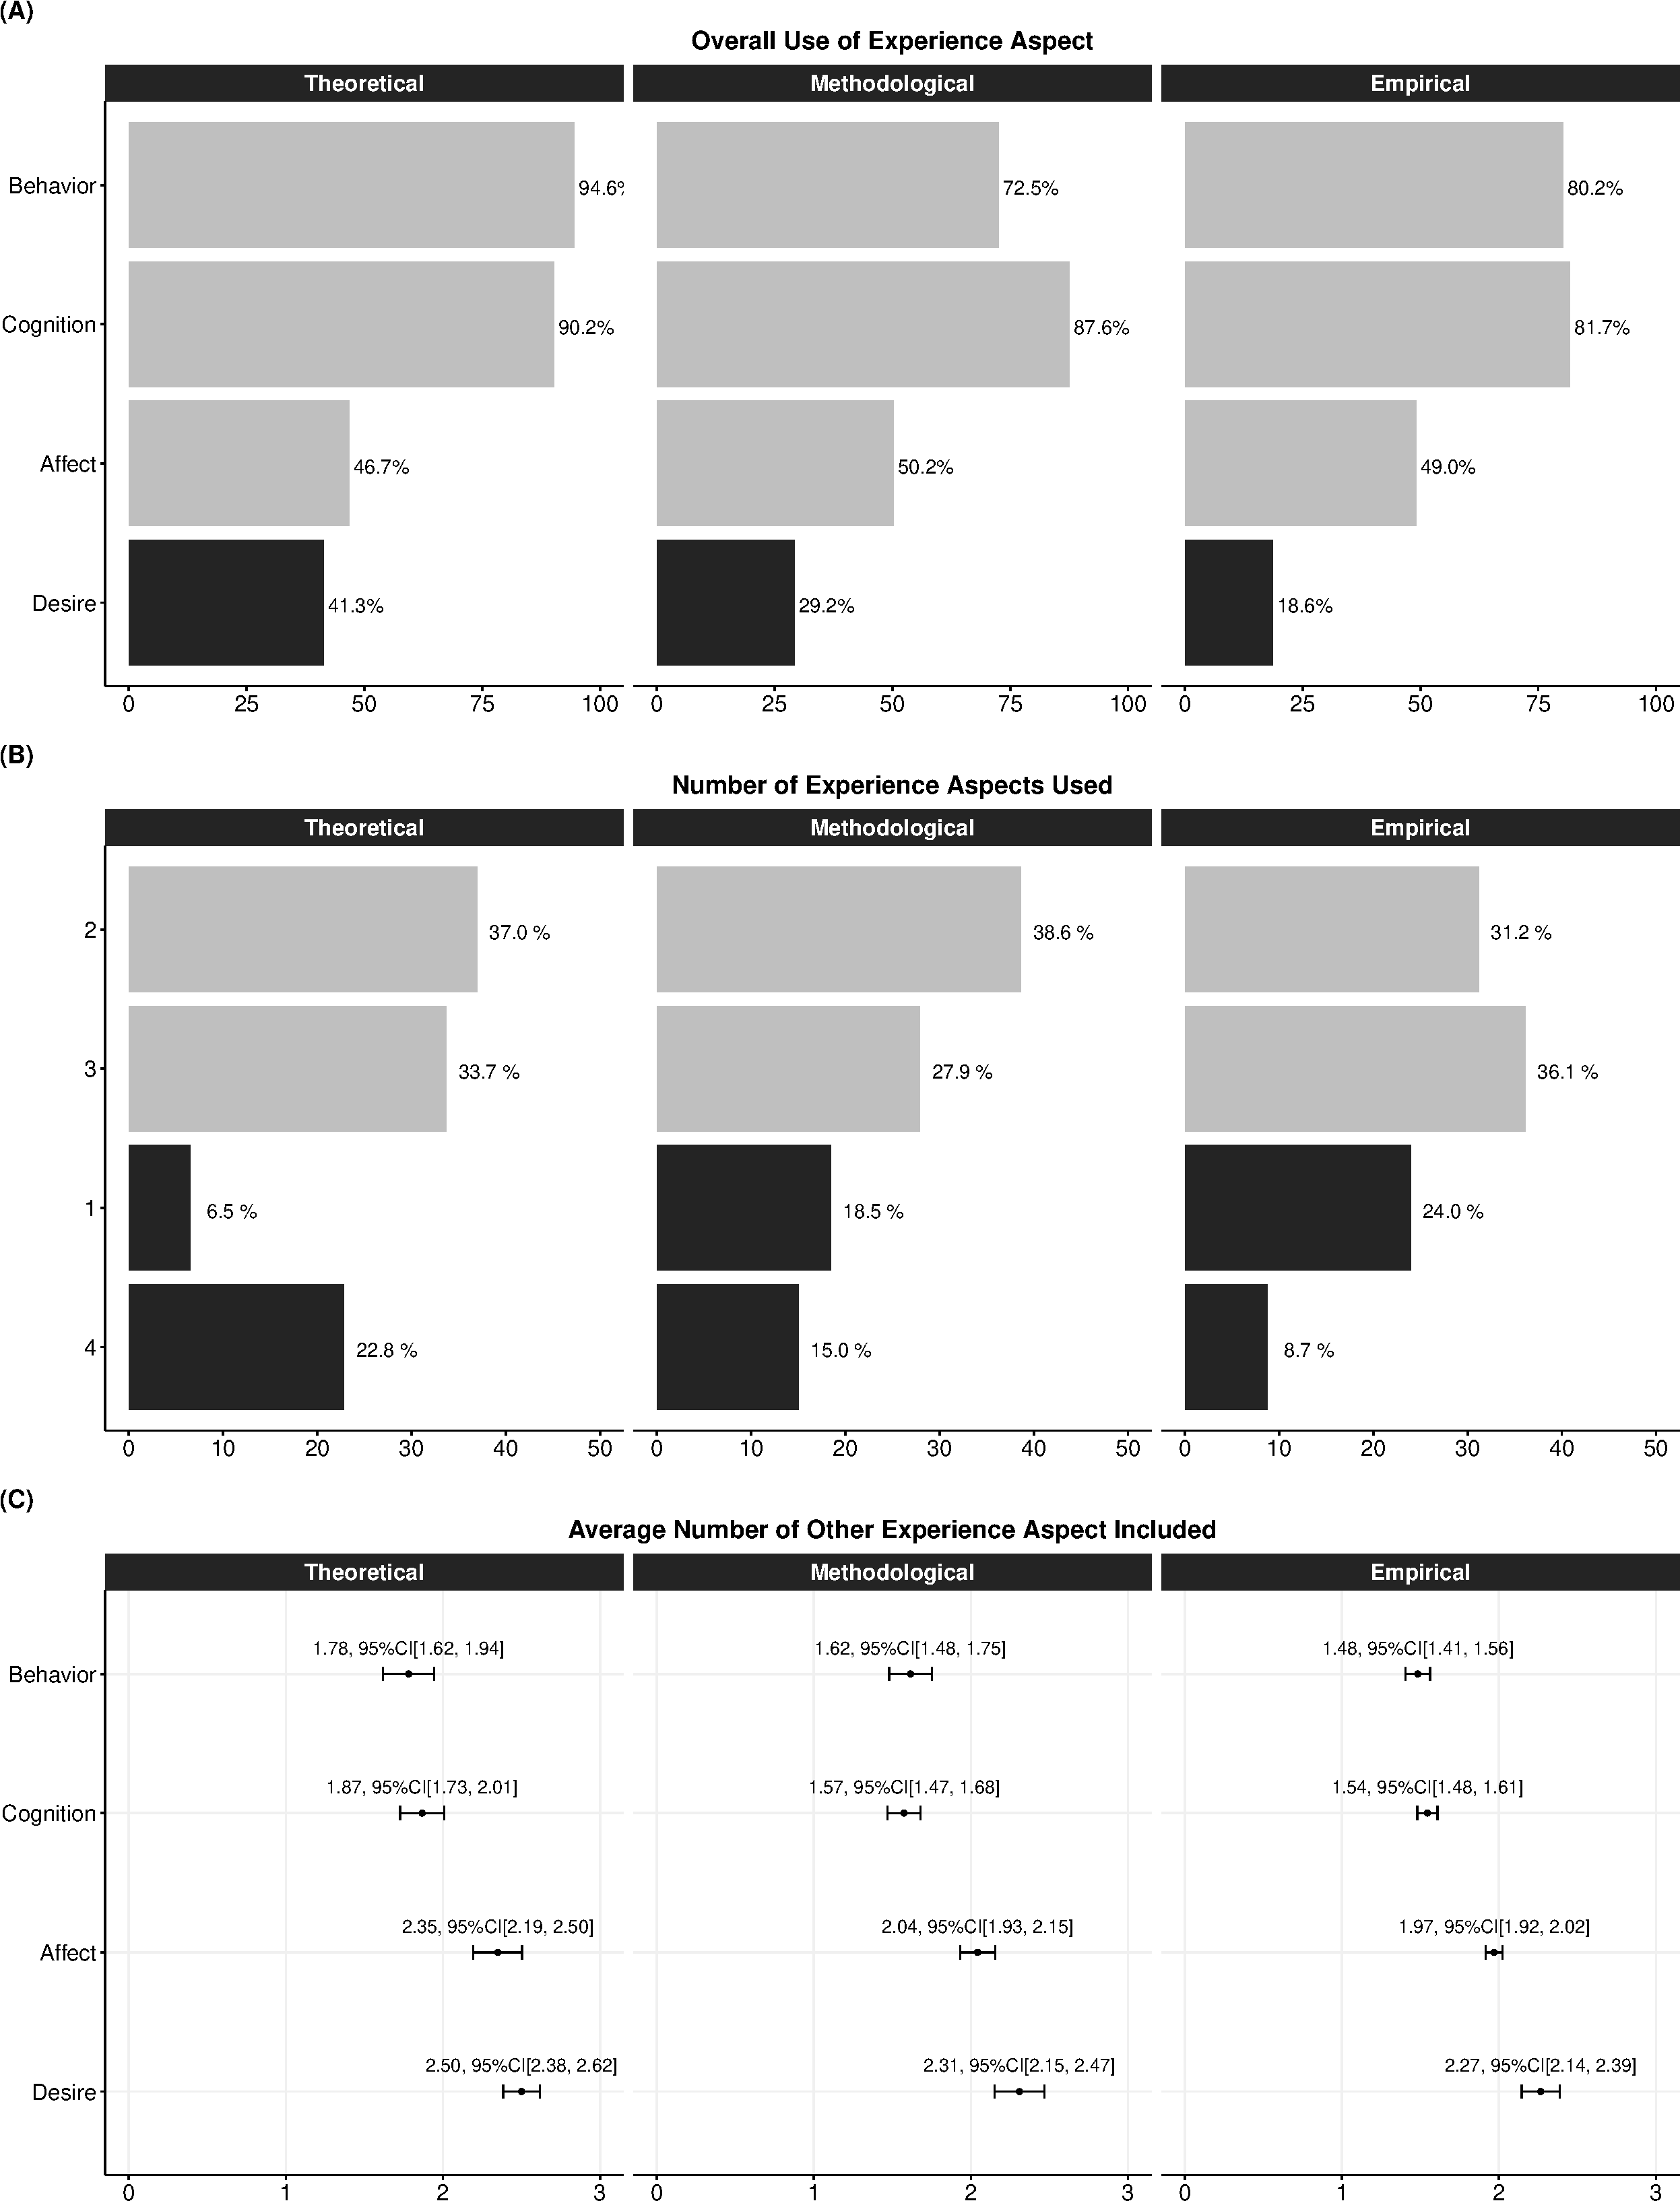
\includegraphics[width=\textwidth]{Figures/LiteratureComparison-1}
\caption*{Note that in (C) within each literature body the aspects are not mutually exclusive (and thus not independent) because scales can include multiple experience aspects.}
\label{fig:LiteratureComparison}
\end{figure}


\section{Discussion}
% Recap: Problem, Aim, Proposal
% Problem:
An enormous variety of aspects of our lives are affected by cultures, the psychological changes we experience when we get into continuous first-hand contact with new cultural patterns (i.e., psychological acculturation) are consequently equally plentiful and diverse.
% Aim:
In order to make sense of past theories and measures of psychological acculturation and to develop new theories and measures, it is thus necessary to build a conceptual framework that allows us to analyze, compare, and understand the individual aspects of psychological acculturation.
% Proposal:
In this paper, we have proposed that taking the fundamental aspects of the human experience (affect, behavior, cognition, and desire) offers a comprehensive and theory-based structure to the psychological acculturation concept (in both theory and application). 

% Emergence from the literature:
Our investigation has utilized a variety of empirical sources and applications that offer support for the applicability of an experience framework in the acculturation field. Firstly, the ABCD experience framework brings together and expands on several key developments within the literature on psychological acculturation. By applying the affect, behavior, cognition, and desire structure across abstract and applied levels of conceptualization, we were able to highlight the complexity and embeddedness of the acculturation process while still offering novel structural nuance in the different phases of the contact with new cultural patterns.

% Literature Review:
% Scales, Empirical, Theories
And secondly, we also applied the experience-based framework in a systematic scoping review of past theoretical, psychometric, and empirical literature on psychological acculturation.
We found that the framework was able to capture a heterogeneous set of theoretical, psychometric, and empirical works. We were able to assess and bring together a broad set of theoretical works and were able to compare conceptualizations between publication fields and across different types of literature. We particularly found that theoretical conceptualizations of psychological acculturation tended to include more ABCD aspects than the psychometric and empirical works, and across all three types of literature, researchers have tended to focus on the more external behaviors and cognitions while the more internal affects and desires have remained understudied, especially in applied empirical works.
    
From our framework development and systematic scoping review, we thus offer several novel insights, which address past conceptual issues.

\begin{enumerate}
\item Our framework highlights that psychological acculturation is based on separate experiences of contact over time. This emphasizes the episodic nature of acculturation, where a majority of the psychological changes are driven by contact events. This focus on the contact episode allows us to conceptually distinguish experiences at different phases of the contact. We see this in the systematic scoping review, where an episodic and contact-focused condition-response-outcome separation was able to organize the past theoretical literature. Additionally, the framework was able to capture cross-sectional as well as longitudinal studies and was relevant to samples prior to and following the migration event (including, prospective migrants). 

\item Because affect, behavior, cognition, and desire broadly capture the human experience \citep[e.g.,][]{Jhangiani2014}, the experience framework comprehensively captures the psychological aspects of acculturation. The framework, thus, offers a theory-driven structure of the concept and its applications while still providing space for the idiosyncratic complexities of the phenomenon. This meant that in our systematic scoping review application very few studies did not capture any experience aspect (e.g., length of residency, or migration status; also see lref{tab:ExclusionsCombined}) and we were arguably able to make meaningful comparisons across a wide variety of contexts and even fields. In short, the ABCD structure offers a common language that opens up the possibility to see where mechanisms are shared or diverging. The broader structure can help us make sense of the differences between individual studies or competing results and as a result lets us more transparently talk about and address the most pressing issues within a given idiosyncratic context.

\item The experience aspects of psychological acculturation highlight a shared humanity across contexts. ABCD structures have been found across cultural contexts because they build on basic human faculties \citep[e.g.,][]{Bhawuk2011}. At the same time, however, the four experience aspects do not prescribe what exactly is being wanted, felt, thought, or done in any given context. The structure instead provides a language to discuss where experiences and psychological mechanisms might be shared or diverging for different contexts. In the scoping review, we were able to assess a wide range of affects, behaviors, cognitions, and desires in acculturation research from more than 315 cultural contexts (see Supplementary Information E).

\item We explain psychological acculturation as a complex phenomenon. Most theoretical works we collected as part of the systematic scoping review conceptualize psychological acculturation as a composite phenomenon that includes multiple aspects of the human experience (affect, behavior, cognition, and desire). This stands in stark contrast to singular research traditions and many empirical operationalizations that have intentionally or unintentionally focused on a single aspect of the psychological acculturation experience \citep[also see][]{Ward2001}.
\end{enumerate}

\subsection{New Research Directions}
From both the development of the experience framework of psychological acculturation and its application in the systematic scoping review, we can thus formulate a number of lessons learned that could guide future work in the field (also see \tblref{tab:SummaryTbl}). We believe that these have a number of broader implications for researchers and practitioners.
For advancing future research projects, the systematic scoping review and the conceptual framework can offer future perspectives for (1) the clarity of conceptualizations, (2) the focus of study or intervention, (3) future empirical tests, and (4) new theoretical predictions. 

% Transfer-ability and comparability: 
% - Additionally, we observed a number of transparency and clarity issues during our systematic scoping review: focus of aspect, operationalization (e.g., items or clear descriptions)
% - Lastly, potential data issues: broad category of migrants considered (e.g., Asian, Spanish-speaking), use of ad-hoc and non-validated scales, focus on clinical outcomes with non-clinical samples.
\paragraph{On transfer-ability and comparability.} Our systematic scoping review highlighted a number of transparency- and transferability issues within the field. In some works, the conceptualization and operationalizations of acculturation remained vague and unexplained (for more information on this issue see Supplemental Materials C and E). Future research should clearly define which experience aspect is focused on and why a particular aspect is (ir)relevant to a specific project. Also more broadly, future research should assess the impact and transfer-ability of sample and measurement decisions, such as recruiting broad categories of migrants (e.g., "Asian", "Spanish-speaking"), the use of ad-hoc and non-validated scales, or the focus on clinical outcomes with non-clinical samples --- all of which were common within the empirical literature.


% Empirical studies:
% - re-iterate the importance of process focus (disconnect theory and empirical)
% - test theories in complexity (disconnect theory and empirical)
% - empirical studies need to investigate affect and desire are needed (highlighted in theories and focus group)
\paragraph{On testing current theories.} We find that theoretical works commonly focus on acculturation as a process that includes multiple experience aspects, while empirical works were considerably more static and narrow in their conceptualization. This gap means that many theoretical models remain empirically untested and many empirical tests are not accurately embedded within theories. Future research should, thus, consider more longitudinal and multi-faceted conceptualizations of acculturation to meaningfully test theoretical models and -predictions in their entirety.

The same static reductionist practices hold true for the conceptualization of culture more broadly. While many theoretical conceptualizations of cultural patterns have pointed to the rich idiosyncrasies of cultural realities, more applied models and empirical studies often fail to capture the multifaceted, interactive, and fluid nature of the cultural patterns migrants (re-)create. Future studies should have a more transparent communication of the cultural patterns involved and more research is needed for contexts where new cultural patterns emerge or several cultural patterns clash.

A similar gap exists in the focus on specific aspects, where affect and desire conceptualizations are highlighted in theoretical works as well as our qualitative study but remain relatively absent in empirical quantitative works. Future empirical studies will thus need to investigate the mechanisms and roles of affective and motivational acculturation.

% Relationships:
% - need to investigate the relationships between different experience aspects. 
% - need to investigate the relationships of experience aspects with other concepts.
\paragraph{On novel theoretical predictions.} Finally, our framework also opens up the possibility to investigate relationships between individual experience aspects of acculturation and relationships of these aspects with other concepts. Future research could, for example, assess whether a certain aspect precedes another or how one aspect might feed back into another. There are plenty (social) psychological theories that speak to the organization of human experiences and offer meaningful predictions of causal pathways for functional elements. For example, when focusing on acculturation behaviors one prediction model might argue that in response to a given interaction situation, cognitions regulate affect and desire to produce adaptive behaviors (cf., cognitive self-regulation theories; \citealp{Panadero2017}; for illustration see \fgrref[A]{fig:NovelModels}). However, a conflicting model might propose that motivations organize cognition and affect, which in turn drive behavior (cf., theory of reasoned goal pursuit; \citealp{Ajzen2019}; also see \fgrref[B]{fig:NovelModels}). It is thus up to future studies to determine which experience aspect causally drives acculturation behaviors. And similar endeavors could help explain emotional, motivational, or cognitive acculturation outcomes. Similarly, the subdivision into experience aspects also allows for more nuanced investigations of these acculturation aspects to other concepts (e.g., does behavioral acculturation have the same impact on health as emotional acculturation?). 

Additionally, because the experience aspects also relate to the structural and embodied aspects of cultural patterns, the aspect separation also allows us to consider contextual affordances. As an example, in most resettlement contexts behavioral acculturation experiences are often much more directly regulated and restricted than motivational, affective, or cognitive acculturation experiences. Laws, policies, and societal interventions that surround occupational or political participation are, for example, often more common than interventions on values, virtues, or emotions \citep[][]{shafir2013}. Within concrete resettlement contexts, considering the four aspects can, thus, for example, help understand differential influences of power inequality and acculturation hurdles \citep[][]{Bhatia2001, Khawaja2019}. 

% Extended Model as theoretical integration
More broadly, the framework also integrates many of the prominent models and theories within the acculturation literature (see \fgrref{fig:ModelContext}). The individual responses in affects, behaviors, cognitions, and desires give space to the fluid and interconnected nature of cultures by capturing the connection between different patterns of shared, embodied, and internal affects, behaviors, cognitions, and desires. As such the framework is consistent with the generalized frameworks \citep[e.g.,][]{Berry2005, Cross1991} and ecological process models within the field \citep[e.g.,][]{Ward2016, Serdarevic2005, Mistry2010}. And by differentiating expected ABCDs prior to contact (i.e., acculturation conditions) from experiences ABCDs during contact (i.e., acculturation response) and after the contact (acculturation outcome) the different temporal stages of an episodic contact experience extend and streamline traditional orientation-outcome models \citep[e.g.,][]{Arends-Toth2006a, TeLindert2008a}. In such a process approach cultural conflict models can additionally address conditions of change \citep[e.g.,][]{Robinson2019} and stress adaptation models can further discern conditions of stress \citep[e.g.,][]{Kim1988, Hajro2019, Sam2006b} between the experience steps. In its structure and approach the framework is also consistent with liminality- \citep[e.g.,][]{Loon2021, Baird2015}, and structuralist approaches \citep[e.g.,][]{Kemppainen2020}.

In its application, the framework might then address the difficulty of quantitative integration --- for example, through meta-analytic reviews. The ABCD experience framework offers both a filter- as well as a moderator solution for new quantitative integration efforts. For specific relationships (e.g., between psychological acculturation and health-seeking behaviors) quantitative reviewers may choose to only select a specific set of experience aspects (e.g., only behavioral acculturation), and if multiple aspects are considered the ABCD structure offers a meaningful moderator variable. 

It is important to note again that distinguishing the four aspects should not reduce the complexity of human experiences. While researchers and lay people are generally able to identify affect, behaviors, cognitions, and desires as distinct aspects of psychological acculturation, it remains important to consider that they often co-occur in psychological concepts and experiences.

\subsection{Practical Implications}
Our framework also offers guidance to practitioners, policymakers, and acculturating individuals. 

%% Use of the framework:
\paragraph{Facilitating intervention focus.} The framework might be of interest to practitioners and policy-makers because it is theory-based and brings together a wide range of past literature. The structured approach might be useful in making clear and informed decisions while still considering the concept in its personal complexity. When considering psychological acculturation practitioners can choose to assess or address emotions and moods (affective acculturation), behaviors and mannerisms (behavioral acculturation), thoughts and cognitions (cognitive acculturation), or needs and desires (motivational acculturation). Whichever selection is made for an application, the framework offers a concise decision-making tool and the review suggests that most theories of acculturation call for a large number of aspects.

\paragraph{Giving agency to the target group.} The experience conceptualization of psychological acculturation is inherently a bottom-up approach to the topic. Taking migration experiences as the starting point highlights the considerations for the lived realities of the researched individuals and communities. Scholars in the traditions of critical research methods have long highlighted the importance of including the participants in the research conceptualization process \citep[e.g.,][]{Kovach2009}. If one uses the experiences of the researched individuals to guide the study or intervention design, one inevitably emphasizes the agency and needs of the community --- lending relevance and ownership of knowledge to the community \citep[e.g., ][]{Schmidt2021}. Using the individual experience as our conceptual foundation reminds us that in clinical and social protection contexts the recipients are human beings with complex experiences. In its application, the four experience aspects thus offer a structure for building humane interventions as well as monitoring and evaluation efforts of such interventions. 

\paragraph{Comprehensive considerations.} Our framework itself, the underlying focus group discussion, as well as the systematic scoping review of the theoretical literature suggest that psychological acculturation is best captured with all four experience aspects of acculturation (i.e., wanting, feeling, thinking, and doing). Efforts that aim to monitor, or address maladaptive acculturation should thus consider the entire broad acculturation experience. Resettlement organizations aiding new migrants may, for example, want to monitor cognitive and behavioral acculturation (e.g, cultural knowledge, or contact behaviors) but should equally consider motivational or emotional acculturation (e.g., unfulfilled competence needs, or feelings of loneliness). 

\begin{table}%[hbt]
\caption{Synthesis Summary and Future Perspectives.}
\label{tab:SummaryTbl} 

\footnotesize

\begin{tabular}{>{\raggedright\arraybackslash}p{0.50\linewidth} 
>{\raggedright\arraybackslash}p{0.50\linewidth}}

\hline 
Critical issues identified in systematic review &
Perspective / Suggestions \\ 
\hline

\vspace{-0.5em} \hangindent=0.55cm 1.~ Theoretical and empirical conceptualizations of psychological acculturation have been diverse and unstructured.  & 
\vspace{-0.5em} The affect, behavior, cognition, desire distinctions could be used to structure acculturation conceptualizations. \\ 

\vspace{-0.5em} \hangindent=0.55cm 2.~ Empirical studies focus on cross-sectional outcome conceptualizations while theories predominantly conceptualize psychological acculturation as a process. & 
\vspace{-0.5em} In empirical works a stronger focus on longitudinal acculturation assessments is needed to congruently test theories empirically. \\ 

\vspace{-0.5em} \hangindent=0.55cm 3.~ Theories include substantially more experience aspects in their conceptualization than empirical studies. & 
\vspace{-0.5em} Empirically, investigations of more acculturation aspects are needed to congruently test theories empirically. \\ 

\vspace{-0.5em} \hangindent=0.55cm 4.~ There has been little empirical focus on emotional and motivational aspects, even though they are important in theories and qualitative discussions. & 
\vspace{-0.5em} To close this gap, empirical studies that investigate the internal aspects of affect and desire are needed. \\ 

\vspace{-0.5em} \hangindent=0.55cm 5.~ The choice of investigated acculturation aspects have often remained elusive in methodological and applied empirical literature. & 
\vspace{-0.5em} For replications, comparisons, and theoretical synthesis, research and intervention choices need to be transparent. Which aspect is focused on? Why is an aspect (ir)relevant to the project? \\ 

\vspace{-0.5em} \hangindent=0.55cm 6.~ Operationalizations and measurements of acculturation have often remained unclear (especially with ad-hoc measures or non-validated modifications and non-disclosed items). & 
\vspace{-0.5em} As long as the field faces conceptual issues, transparency in measurement would be important. Either items or clear content descriptions should be available. And research should assess the impact of non-validated scales.\\ 

\vspace{-0.5em} \hangindent=0.55cm 7.~ In theoretical and empirical work, experience aspects are commonly considered independently. & 
\vspace{-0.5em} There is a need to investigate the relationships between different experience aspects. \\ 

\vspace{-0.5em} \hangindent=0.55cm 8.~ Theories have independently been applied to different aspects (e.g., behavioral or cognitive orientations), but effects have rarely been compared across aspects.  & 
\vspace{-0.5em} To synthesize past research, relationships of acculturation with other concepts need to be compared where acculturation has been conceptualized within different experience aspects. \\ 

\vspace{-0.5em} \hangindent=0.55cm 9.~ Psychological and cultural adaptation (as a form of acculturation) have often been conceptualized inconsistently. & 
\vspace{-0.5em} Future investigations and interventions could consider functionality and adaptation within each experience aspect. \\ 

\vspace{-0.5em} \hangindent=0.65cm 10. The normative aim of acculturation conceptualizations are often unclear (e.g., does the conceptualization aim to benefit an individual or society?). & 
\vspace{-0.5em} There is a need to discuss the normative expectations of acculturation conceptualizations within empirical and theoretical work \citep[e.g.,][]{Ager2008a}. \textit{Maybe move to conceptualization (point 5)?} \\ 

\vspace{-0.5em} \hangindent=0.65cm 11. The non-dominant target group has often been defined very broadly (e.g., any migrant, Asia, Spanish-speaking, third world). & 
\vspace{-0.5em} Research questions, conceptualizations, and measurements concerning acculturation should be specific to all considered cultural contexts or should be transferable across all considered cultural contexts. \\ 

\vspace{-0.5em} \hangindent=0.65cm 12. We identified \nTheo\ (mostly independent) theoretical works. & 
\vspace{-0.5em} Future research should assess the possibility of theoretical synthesis. The experience framework might offer a conceptual lens for such a synthesis.\\ 

\vspace{-0.5em} \hangindent=0.65cm 13. Acculturation measures are often validated within specific cultural contexts but are applied within other cultural contexts. & 
\vspace{-0.5em} Future research needs to investigate the potential impact of measure transference. \textit{Maybe move to measurement (point 6)?} \\ 

\vspace{-0.5em} \hangindent=0.65cm 14. Empirical work has had a strong focus on clinical outcomes but utilized few clinical samples. & 
\vspace{-0.5em} \textit{probably drop this.} \\ 

\hline

\end{tabular}
\end{table}


\begin{figure}[ht!]
\centering
    \caption{Novel Prediction Models with Behavioral Focus based on the Acculturation Experience Framework. Two examples of (A) a cognitive regulation model and (B) a fundamental needs model.}
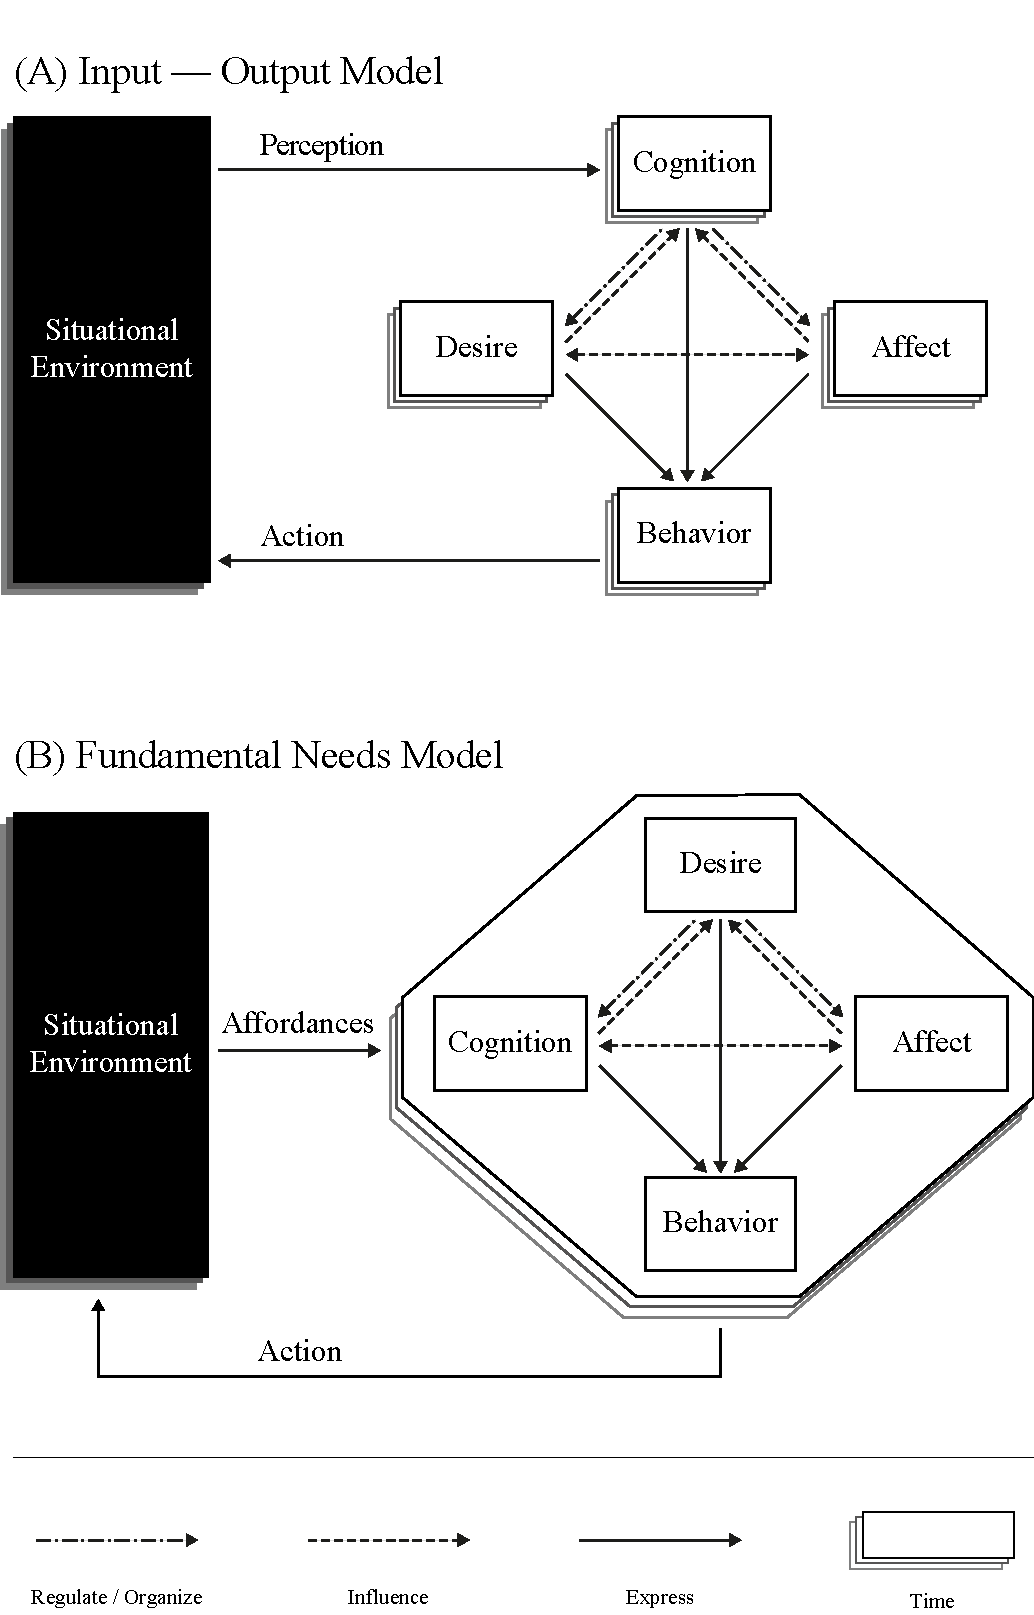
\includegraphics[width=0.9\textwidth]{Figures/NovelPredictionsBehaviorTime.pdf}
\label{fig:NovelModels}
\end{figure}

\subsection{Constraints on Generality, Positionality, and Citations}
Yet, as with any large-scale conceptual undertaking, the framework and this review study are not without limitations. Notably, the framework exclusively focuses on the psychological acculturation process. This has been the explicit focus of our efforts but this also means that non-psychological aspects such as biological, cultural, or societal changes are not captured directly but only to the extent to which they impact the experiences of the involved people. Future work might want to integrate these different levels of group and individual, body and mind \citep[e.g.,][]{Eronen2021}. 

Another point that we have thus far mostly disregarded is the role of the migration context. While we have argued that the framework structure (i.e., the four experience aspects) is relevant across contexts, the lived experiences are often fundamentally influenced by their context and environment. Three major contextual factors often found within the literature are the cultural patterns, the contact situation or life domain, and the interacting individuals. As we already alluded to during the framework development, all of these contextual elements will likely have a profound impact on the experience of affects, behaviors, cognitions, and desires. Cultural patterns, such as laws or norms, individual differences, such as personality or age, but also situational differences in how public or private the acculturation experience is are all likely intermingled with the individual experience aspects. This means that especially within more applied research projects such contextual considerations will be meaningful predictors of individual and group differences (for a first discussion of these contextual factors within our systematic scoping review, see Supplemental Material E). 

Beyond the more methodological constraints, we would also like to briefly address the generality of the samples included in the systematic scoping review. We included \nMeth \, studies in the psychometric literature, and \nEmp \, studies from the broader empirical literature. While the studies jointly included 43 host societies, and 118 societies of origin (with a total of 315 unique combinations), for both bodies of literature an overwhelming amount of studies were conducted in `western' countries --- Western Europe (e.g., The Netherlands, United Kingdom, Germany, Italy, Spain), Australasia (Australia, New Zealand), Russia, and Israel. As an example, 126 scales were validated for a U.S. American resettlement context, and 324 of the included empirical studies focused on migrants arriving in North America (i.e., U.S. and Canada). When it came to the migrants' country of origin, a majority of studies were indifferent to migrants' background and simply recruited any consenting migrant ($N_{psychometric}=$ 53, $N_{empirical}=$ 108), or recruited broad category of migrants (e.g., LatinX or Hispanic: $N_{psychometric}=$ 22, $N_{empirical}=$ 67; Asian: $N_{psychometric}=$ 10, $N_{empirical}=$ 26). Among the studies, that recruited participants from specific cultural backgrounds, Mexican, Chinese, and South Korean migrants were recruited most frequently. To address the lack of research on migration to non-western countries, we additionally searched for and included qualitative studies and grounded theories, which unfortunately are often the only works to engage with understudied communities. However, even with these inclusions and additional search strategies, the field remains Western-centric. While we sought to build a conceptual structure that focuses on shared basic capacities, the framework did emerge from the literature and the included studies remain a constraint of the scoping review.

Next to the more formal limitations of scope and methodology, we would like to situate our framework, its application, and its limitations more broadly. For such a reflection, it is essential to expand on how our own beliefs, judgments, and practices have shaped the development of the framework and its application. In the most practical sense, the extensive, multiyear efforts of this project grew out of a research-NGO collaboration and an academic frustration. The conceptual question of what we mean by `acculturation' and how we should assess it was initially raised during this local collaboration with a refugee resettlement organization. However, trying to make sense of the heterogeneous acculturation conceptualizations within the academic literature to develop more sustainable metrics for practitioners, initially highlighted that we miss an overarching manner in which we make sense of the concept. 

Our own approach to this question was certainly guided by our own backgrounds and past experiences. The main author has been working with forced migrants for over 10 years in three countries around the world --- in refugee resettlement programs under the UNHCR, as a volunteer, language teacher, and integration coach with several smaller and larger migration organizations. Additionally, three of the five authors were first-generation migrants at the time of the writing of this article. Our own, decidedly applied experiences with the importance and diversity of psychological acculturation, have assuredly influenced our research process. Most notable are our choices to take a phenomenological perspective and our focus on the migrant minority perspective in understanding the psychological mechanisms of acculturation. Taking a bottom-up and migrant-centered focus was fundamental to our approach.

Similarly, all five authors have contributed a unique view to this project in terms of their academic background. The author team consists of two social psychologists but also includes a clinical-developmental, and an organizational psychologist, as well as a methodologist and statistician. The team not only exemplifies the diversity of fields that are affected by questions of acculturation but also brought about the basic structure of the framework we suggest. Making sense of the qualitative responses and the past conceptual literature, the ABCD division of the human experience is arguably a multidisciplinary structure that coherently conformed to the bodies of literature we were familiar with prior to the systematic scoping review. 

On a more abstract level, we would like to address some of the ontological and epistemological influences that have shaped our approach. Our research question and conceptual framework are fundamentally motivated by our structuralist ontology. Here we follow the stance that others like \citet[][]{Berry2009a} have taken, where we argue that affect, behavior, cognition, and desire are basic human capacities. Importantly, in our view, this does not imply cultural determinism or deny cultural and individual diversity. While we argue that everyone has the capacity for emotions, we do not argue that this determines which emotions an individual will feel at any given moment. By extension, the same holds true for affective acculturation, where we argue for its structural existence but not a culturally universal content. Similarly, the way in which we sought to validate our framework is arguably the result of our own empiricist epistemological background. In particular, we chose to systematically collect past academic literature and extracted conceptual aspects to apply the framework. Thus, while we have included some qualitative review elements, our efforts were mainly deductive and had a hypothesis-testing rather than hypothesis-generating quality in their application.

Finally, we would like to speak to the diversity of the scholars we cite and who form the body of the literature we worked with. To assess the broadest level of structural bias within the work we cite, we used a `cleanBib` pipeline developed by \citet{zhou2022}. The Python program allowed us to analyze the first/last author pairs in our bibliography entries. The program relies on probabilistic gender and ethnicity assignments based on the authors' names. The predictive validity of both the underlying Gender API \citep[][]{sebo2021} and the name ethnicity predictor has been well-established \citep[][]{ambekar2009, sood2018}. For both measurements, we excluded self-citations of the first and last authors of this current paper. For the works cited within this manuscript, we found scholars were 22.88\% woman(first)/woman(last), 15.29\% man/woman, 15.44\% woman/man, and 46.38\% man/man. Additionally, our references contain 17.29\% author of color (first)/author of color(last), 14.40\% white author/author of color, 15.75\% author of color/white author, and 52.57\% white author/white author. Compared to the full set of works that were included in the scoping review, our references match the patterns of the theoretical literature. 

Interestingly, when we compared the distributions across the three bodies of theoretical, psychometric, and broader empirical literature, we saw that women and people of color were less frequently authors of theoretical literature but were substantially better represented within the psychometric and the empirical literature (empirical gender: 40.18\% woman/woman and 25.68\% man/man; ethnicity: 23.72\% author of color/author of color and 34.88\% white author/white author). This might be due to the larger sample sizes or represent a broader inequality within the field. Beyond the limitations of the method we employed here\footnote{Gender prediction via this method may be limited to the names, pronouns, and social media profiles, which have been used to build the data set. Additionally, the method is unable to account for intersex, non-binary, or transgender individuals. Similarly, the method's predictive accuracy for race and ethnicity may be restricted by the use of names and how well they are represented in the Florida Voter Data. The approach may not account for Indigenous and mixed-race authors or individuals facing ambiguous racial or ethnic identification. Differential biases may also arise due to such ambiguity.}, it should also be noted that privilege and discrimination are layered, multidimensional, and often intersectional. Important additional markers of such inequalities include access to funding, the journal tier, and the research institution, all of which are readily available for most published works and future research should seek to assess and address the inequalities within the field more rigorously. 

\subsection{Conclusions}
By building on recent developments within the field, we suggest a conceptual framework of psychological acculturation, utilizing the affect-behavior-cognition-desire aspects of human experiences. We showcase the structuring and comparative utility by applying the framework in a systematic scoping review of the past theoretical, psychometric, and empirical literature. We find that the framework is able to comprehensively structure past works (e.g., few articles did not fit the ABCD conceptualization), identify gaps within the literature (e.g., a crucial disconnect between theory and empirical practice), and is able to assist in future theoretical and applied conceptualizations (e.g., novel predictions and interventions). As such, the framework provides a robust starting point and a useful tool for both researchers and practitioners.

%\newpage

\printbibliography

\appendix

\section{Search Strategy}
\label{app:AppendixSearchStrategy}

To assess the past empirical and theoretical literature on psychological acculturation, we performed a systematic literature review. We first read seminal and review works within the field \citep[including,][]{Ward2019, Berry1997b, Berry2003, Szapocznik1978, Sam2006a, Rudmin2003a}. Based on our reading of the literature, we designed a comprehensive literature search strategy in an iterative fashion. 

For the empirical work on acculturation, we performed a literature search on March 4\textsuperscript{th}, 2020 and February 14\textsuperscript{th}, 2021, within the ``APA PsycINFO'' bibliographic databases using the EBSCO\textit{host} provider. The databases also included the PsycARTICLES, PsycBOOKS, and PsycCRITIQUES databases as well ProQuest Dissertations with psychological relevance. The second literature search included alternate terms used less frequently to describe what we mean with psychological acculturation, including "transculturation" and "cultural transition". Additionally, the second search removed limiter terms that could have exclude interdisciplinary investigations and focused on human participants.

For the theoretical literature performed an additional, more specific, search of the same databases as well as the Web of Science Core Collection using the Clarivate Analytics provider on March 3\textsuperscript{rd}, 2021.

In designing our search strategy we used an adapted version of the `SPIDER' research tool \citep[e.g.,][]{Cooke2012}. We utilized the \textit{Evaluation} element mainly to exclude articles that were not relevant to the search. The exact search terms used are listed in \tblref{tab:SearchStrategiesTab} below.

\begin{table}
\caption{Search Strategy Cultural Adaptation Review}
\label{tab:SearchStrategiesTab} 
\begin{tabular}{ll}
\hline
Element & Search Terms \\ 
\hline \\ [-0.5em]

% Sample
Sample & 
    (Immigration OR migration OR migrant OR immigration OR refugee) \\ 
    \\ [-0.25em]
    
% Phenomenon of Interest
\begin{tabular}[t]{@{}l@{}}Phenomenon \\of Interest\end{tabular} & 
    \begin{tabular}[t]{@{}l@{}}(acculturation OR enculturation OR transculturation OR \\
    assimilation OR "social integration" OR "cultural adaptation" OR \\
    "cultural adjustment" OR "cultural transition")\end{tabular}  \\ 
    \\ [-0.25em]
    
% Design
Design & 
    \begin{tabular}[t]{@{}l@{}}("measurement tool" OR scale OR instrument OR \\
    questionnaire OR survey OR definition OR inventory)\end{tabular}  \\ 
    \\ [-0.25em]
    
% Evaluation
Evaluation & 
    \begin{tabular}[t]{@{}l@{}}NOT (parent* OR college OR resilience OR treatment OR \\
    intervention OR therapy)\end{tabular}  \\ 
    \\ [-0.25em]
    
% Research Type
Research type * & 
    (quantitative OR qualitative OR "mixed method") \\ [0.75em] 
    \hline

% Note
\multicolumn{2}{l}{* This element was ultimately dropped because it was too sensitive in PsycInfo.}
\end{tabular}
\end{table}

\begin{figure}
\centering
\caption{PRISMA Diagrams for the Theoretical, Psychometric, and Empirical Literature.}
\makebox[\textwidth]{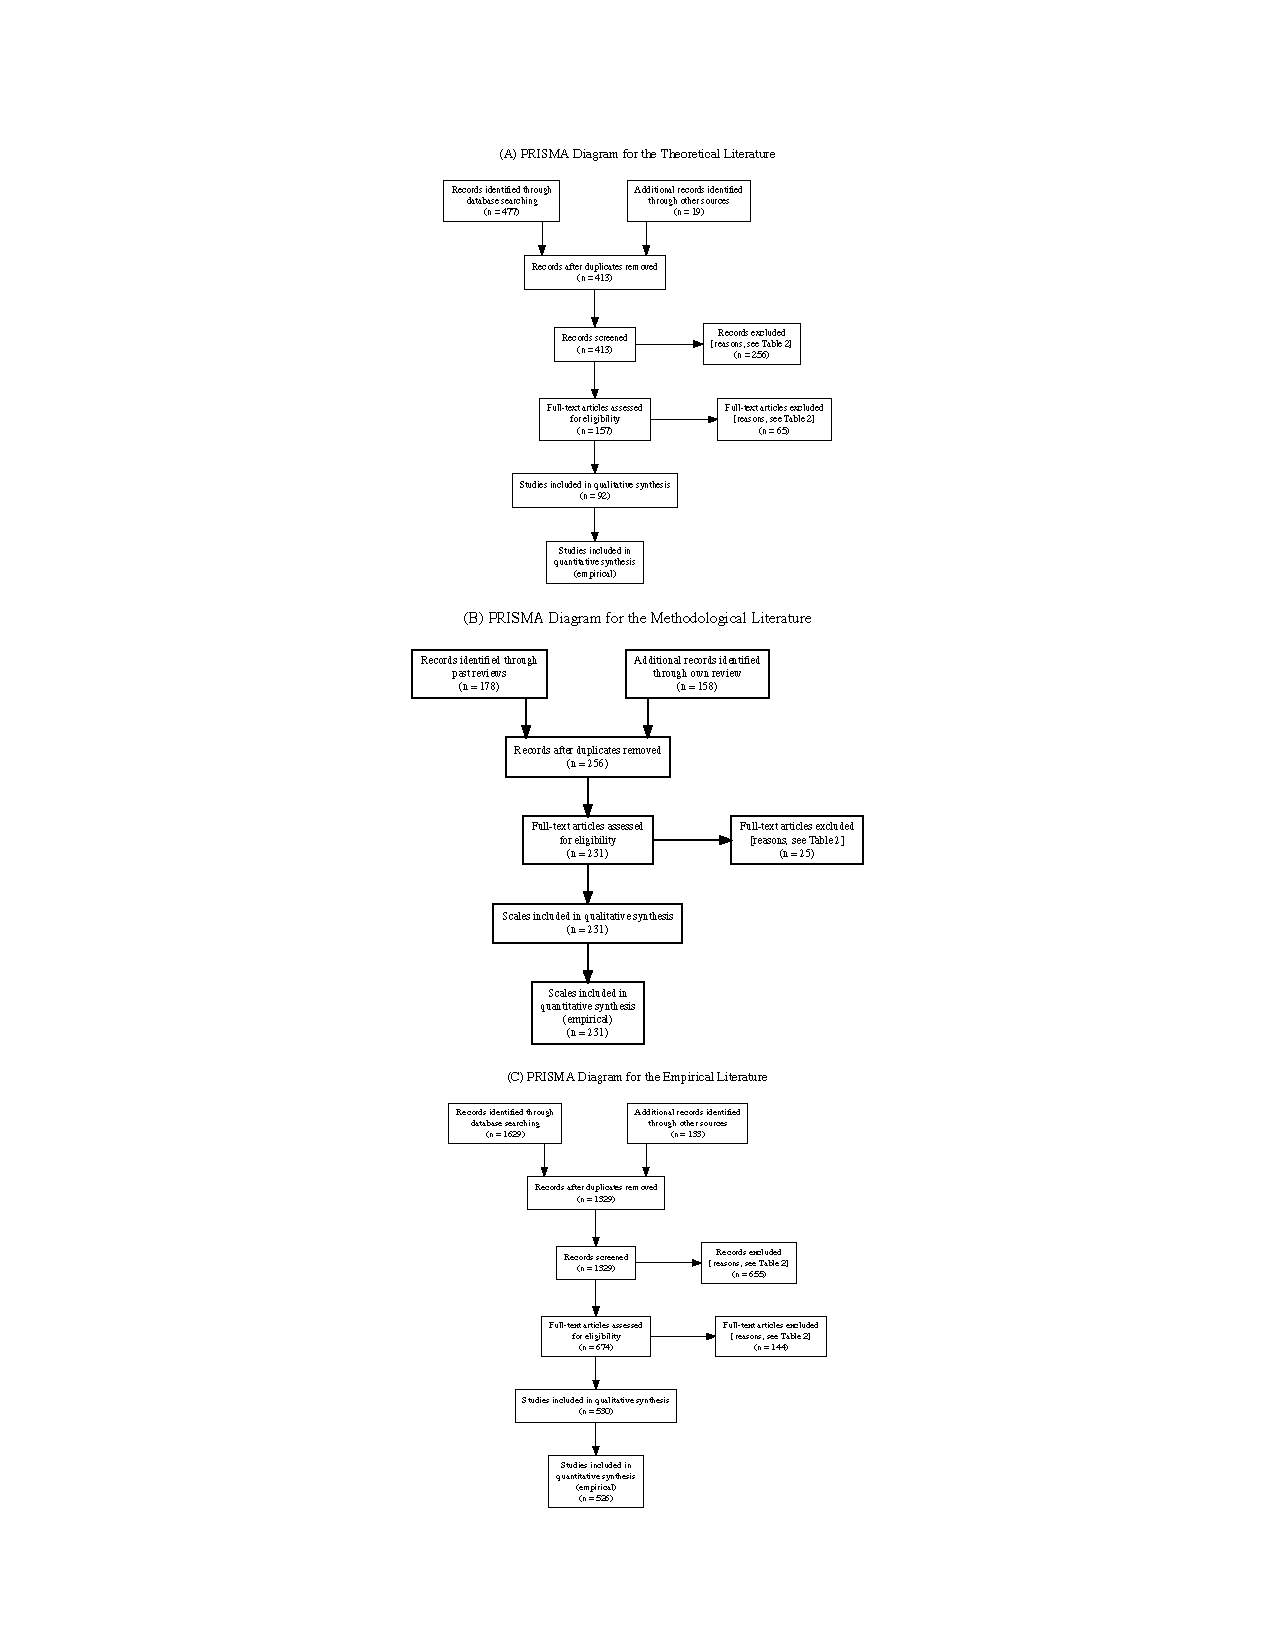
\includegraphics[width=\paperwidth, trim={0 0 0 1.5cm}]{Figures/PrismaCombined-1}}
\label{fig:PrismaCombined}
\end{figure}


\end{document}

%% 
%% Copyright (C) 2019 by Daniel A. Weiss <daniel.weiss.led at gmail.com>
%% 
%% This work may be distributed and/or modified under the
%% conditions of the LaTeX Project Public License (LPPL), either
%% version 1.3c of this license or (at your option) any later
%% version.  The latest version of this license is in the file:
%% 
%% http://www.latex-project.org/lppl.txt
%% 
%% Users may freely modify these files without permission, as long as the
%% copyright line and this statement are maintained intact.
%% 
%% This work is not endorsed by, affiliated with, or probably even known
%% by, the American Psychological Association.
%% 
%% This work is "maintained" (as per LPPL maintenance status) by
%% Daniel A. Weiss.
%% 
%% This work consists of the file  apa7.dtx
%% and the derived files           apa7.ins,
%%                                 apa7.cls,
%%                                 apa7.pdf,
%%                                 README,
%%                                 APA7american.txt,
%%                                 APA7british.txt,
%%                                 APA7dutch.txt,
%%                                 APA7english.txt,
%%                                 APA7german.txt,
%%                                 APA7ngerman.txt,
%%                                 APA7greek.txt,
%%                                 APA7czech.txt,
%%                                 APA7turkish.txt,
%%                                 APA7endfloat.cfg,
%%                                 Figure1.pdf,
%%                                 shortsample.tex,
%%                                 longsample.tex, and
%%                                 bibliography.bib.
%% 
%%
%% End of file `./samples/longsample.tex'.
